\documentclass{beamer}
\usetheme{Madrid}
\setbeamertemplate{navigation symbols}{}

\usepackage{amsmath}
\usepackage{graphicx}
\usepackage{multicol}
\usepackage{multirow}
\usepackage{array}

\usepackage{tikz}
\usetikzlibrary{shapes.geometric, shapes.misc, arrows}
\usetikzlibrary{calc}
\usetikzlibrary{graphs}
\usetikzlibrary{positioning}
\usetikzlibrary{decorations.pathreplacing}

\usepackage{multirow}  % use tables with columns stretching over multiple rows
\usepackage{booktabs}

\usepackage{pgfplots}
\pgfplotsset{compat=1.18}

\pgfplotsset{
  report_style/.style={
    legend style={draw=none, font=\small},
    legend cell align=left,
    legend pos=north east,
    ylabel style={align=center, font=\bfseries\boldmath},
    xlabel style={align=center, font=\bfseries\boldmath},
    x tick label style={font=\bfseries\boldmath},
    y tick label style={font=\bfseries\boldmath},
    scaled ticks=false,
    every axis plot/.append style={thick},
  },
}

\usepackage[justification=centering]{caption}
\usepackage{subcaption}

\usepackage{xurl}

% default path to images and other assets
\graphicspath{{../assets/}}

% disable wrapping
\tolerance=1
\emergencystretch=\maxdimen
\hyphenpenalty=10000
\hbadness=10000

% number figure caption
\setbeamertemplate{caption}[numbered]

% display bib label in references
\setbeamertemplate{bibliography item}{\insertbiblabel}
\setbeamertemplate{bibliography entry title}{}
\setbeamertemplate{bibliography entry location}{}
\setbeamertemplate{bibliography entry note}{}

% \newcommand{\fall}[1]{\quad \textcolor{red}{#1}}
\newcommand{\aligncolor}{teal}
\newcommand{\src}[1]{#1^{src}}
\newcommand{\tgt}[1]{#1^{tgt}}
\newcommand{\floor}[1]{\left\lfloor #1 \right\rfloor}
\newcommand{\ceil}[1]{\left\lceil #1 \right\rceil}
\newcommand*\quot[2]{{^{\textstyle #1}\big/_{\textstyle #2}}}
\DeclareMathOperator*{\argmax}{arg\,max}

% Metadata
% ------------------------
\title[XLNER]{Formalization of natural language processing tasks as optimization problems}
\subtitle{Master thesis}

\author[Oleh Shkalikov]{Oleh Shkalikov\texorpdfstring{ (5102818)
    \\[0.7em]{\small Supervisor: Jannik Irmai}
\\{\small Reviewers: Prof. Dr. Bjoern Andres, Prof. Dr. Simon Razniewski}}{}}

\institute[TU Dresden]{TU Dresden}

\date{January 24, 2025}

\begin{document}

\frame{\titlepage}

% \begin{frame}
%   \frametitle{Table of contents}
%   \tableofcontents
% \end{frame}

\section{Introduction}

\begin{frame}
  \frametitle{Named Entity Recognition}

  \begin{block}{What is NER?}
    Predict a class for every word and then aggregate entities, i.e.
    continuous sequences of words that belong to a single object.
  \end{block}
  % \vspace*{0.75cm}
  \begin{figure}[ht]
    \centering
    \begin{tikzpicture}[node distance=-0.1,
        every node/.style={text centered,
          text height=2ex,
          text depth=.25ex,
        },
        loc/.style={fill=orange!30, rounded rectangle, label={[anchor=center,font=\tiny\bfseries\sffamily]above:####1-LOC}},
        per/.style={fill=green!30, rounded rectangle, label={[anchor=center,font=\tiny\bfseries\sffamily]above:####1-PER}},
        O/.style={rounded rectangle, label={[anchor=center,font=\tiny\bfseries\sffamily]above:O}}
      ]

      \node[per={B}, rounded rectangle east arc=none](Mark){Mark};
      \node[per={I}, rounded rectangle west arc=none, right=of Mark](Twain){Twain};
      \node[O, right=of Twain](was){was};
      \node[O, right=of was](born){born};
      \node[O, right=of born](in){in};
      \node[loc={B}, right=of in]{Florida};
    \end{tikzpicture}
    \caption{Example of NER labeling in IOB2 format}
    \label{fig:ner}
  \end{figure}

  \begin{exampleblock}{Why NER is Important?}
    NER is a building block of various systems such as information retrieval,
    question answering, search engines, and more.
  \end{exampleblock}
\end{frame}

\begin{frame}
  \frametitle{Issues of multilingual NER}

  \begin{alertblock}{}
    The lack of (labelled) data is the main problem in multilingual NER!
  \end{alertblock}

  \vspace*{0.5cm}

  Number of datasets for the token classification task on the HF Hub:
  \begin{itemize}
    \item English: 462
    \item German: 91
    \item Ukrainian: 21
    \item Estonian: 22
    \item Thai: 11
    \item Upper Sorbian: 8
  \end{itemize}
\end{frame}

\section{Related works}

\begin{frame}
  \frametitle{Classification of approaches to XLNER}

  \begin{figure}
    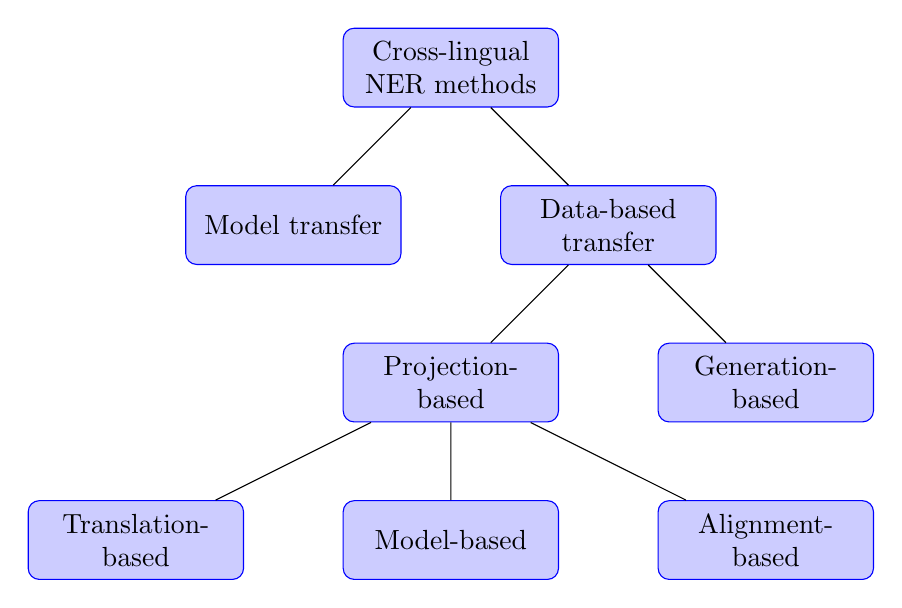
\begin{tikzpicture}[nodes={rectangle, rounded corners,
          minimum width=2cm, text width=2.5cm, minimum height=1cm,
        text centered, draw=blue, fill=blue!20},
        sibling distance=4cm, level distance=2cm,
      ]
      \node {Cross-lingual NER methods}
      child {node(a){Model transfer} edge from parent}
      child {node(b){Data-based transfer}
        child {node(d){Projection-based}
          child {node(e){Translation-based}}
          child {node(e){Model-based}}
          child {node(e){Alignment-based}}
        }
        child {node(c){Generation-based} edge from parent}
      };
    \end{tikzpicture}
  \end{figure}
\end{frame}

\begin{frame}
  \frametitle{Model transfer}
  \begin{columns}[t]
    \begin{column}{0.5\textwidth}
      \begin{block}{General idea}
        Transfer knoweledge from high- resource language to
        all languages
      \end{block}

      \begin{itemize}
        \item Encoder-only: BERT-like
        \item Full Transformer: mT5, etc
        \item Decoder-only: LLMs
          \begin{itemize}
            \item Prompting
            \item Constrained Generation
            \item Zero-/Few- shot
          \end{itemize}
      \end{itemize}
    \end{column}
    \begin{column}{0.5\textwidth}  %%<--- here
      \begin{table}
        \scalebox{0.75}{
          \begin{tabular}{lr|lr}
            \toprule
            Language & Percent & Language & Percent \\
            \midrule
            en & 89.70 & uk & 0.07 \\
            unknown & 8.38 & ko & 0.06 \\
            de & 0.17 & ca & 0.04 \\
            fr & 0.16 & sr & 0.04 \\
            sv & 0.15 & id & 0.03 \\
            zh & 0.13 & cs & 0.03 \\
            es & 0.13 & fi & 0.03 \\
            ru & 0.13 & hu & 0.03 \\
            nl & 0.12 & no & 0.03 \\
            it & 0.11 & ro & 0.03 \\
            ja & 0.10 & bg & 0.02 \\
            pl & 0.09 & da & 0.02 \\
            pt & 0.09 & sl & 0.01 \\
            vi & 0.08 & hr & 0.01 \\
            \bottomrule
          \end{tabular}
        }
        \caption{Language distribution in pretraining data of the Llama2 with percentage above 0.005\%}
      \end{table}
    \end{column}
  \end{columns}
\end{frame}

\begin{frame}
  \frametitle{Projection-based pipeline}

  \begin{figure}
    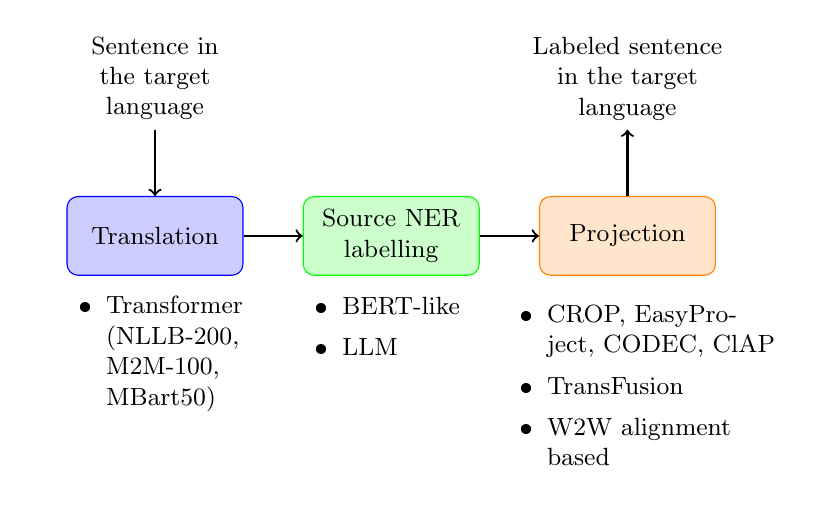
\begin{tikzpicture}[
        nodes={text width=2cm, minimum height=1cm,
        text centered, font = {\small}},
        step_style/.style={rectangle, rounded corners},
        text_style/.style={text width=3cm},
      node distance=3cm]

      % \draw[dashed] (1.5, 0) -- (1.5, 7);

      \node (orig_text) at (0,0) {Sentence in the target language};
      \node[step_style, draw=blue, fill=blue!20, below of=orig_text, yshift=1cm] (fwd_trans) {Translation};
      \node[step_style, draw=green, fill=green!20, right of=fwd_trans] (source_ner) {Source NER labelling};
      \node[step_style, draw=orange, fill=orange!20, right of=source_ner] (proj) {Projection};
      \node[above of=proj, yshift=-1cm, text width=2.5cm] (labeled_orig) {Labeled sentence in the target language};

      \node[text_style, below of=fwd_trans, yshift=1.5cm] {\vbox {
          {
            \begin{itemize}
              \item Transformer (NLLB-200, M2M-100, MBart50)
            \end{itemize}}}};
      \node[text_style, below of=source_ner, yshift=1.85cm] {\vbox {
          {
            \begin{itemize}
              \item BERT-like
              \item LLM
            \end{itemize}}}};
      \node[text_style, below of=proj, yshift=1.1cm, text width=3.8cm] {\vbox {
          {
            \begin{itemize}
              \item CROP, EasyProject, CODEC, ClAP
              \item TransFusion
              \item W2W alignment based
            \end{itemize}}}};

      \draw[->, thick] (orig_text) -- (fwd_trans);
      \draw[->, thick] (fwd_trans) -- (source_ner);
      \draw[->, thick] (source_ner) -- (proj);
      \draw[->, thick] (proj) -- (labeled_orig);
    \end{tikzpicture}
    \caption{General scheme of projection-based pipelines}
  \end{figure}
\end{frame}

\begin{frame}
  \frametitle{Translation-based projection: CROP and EasyProject}
  \begin{figure}
    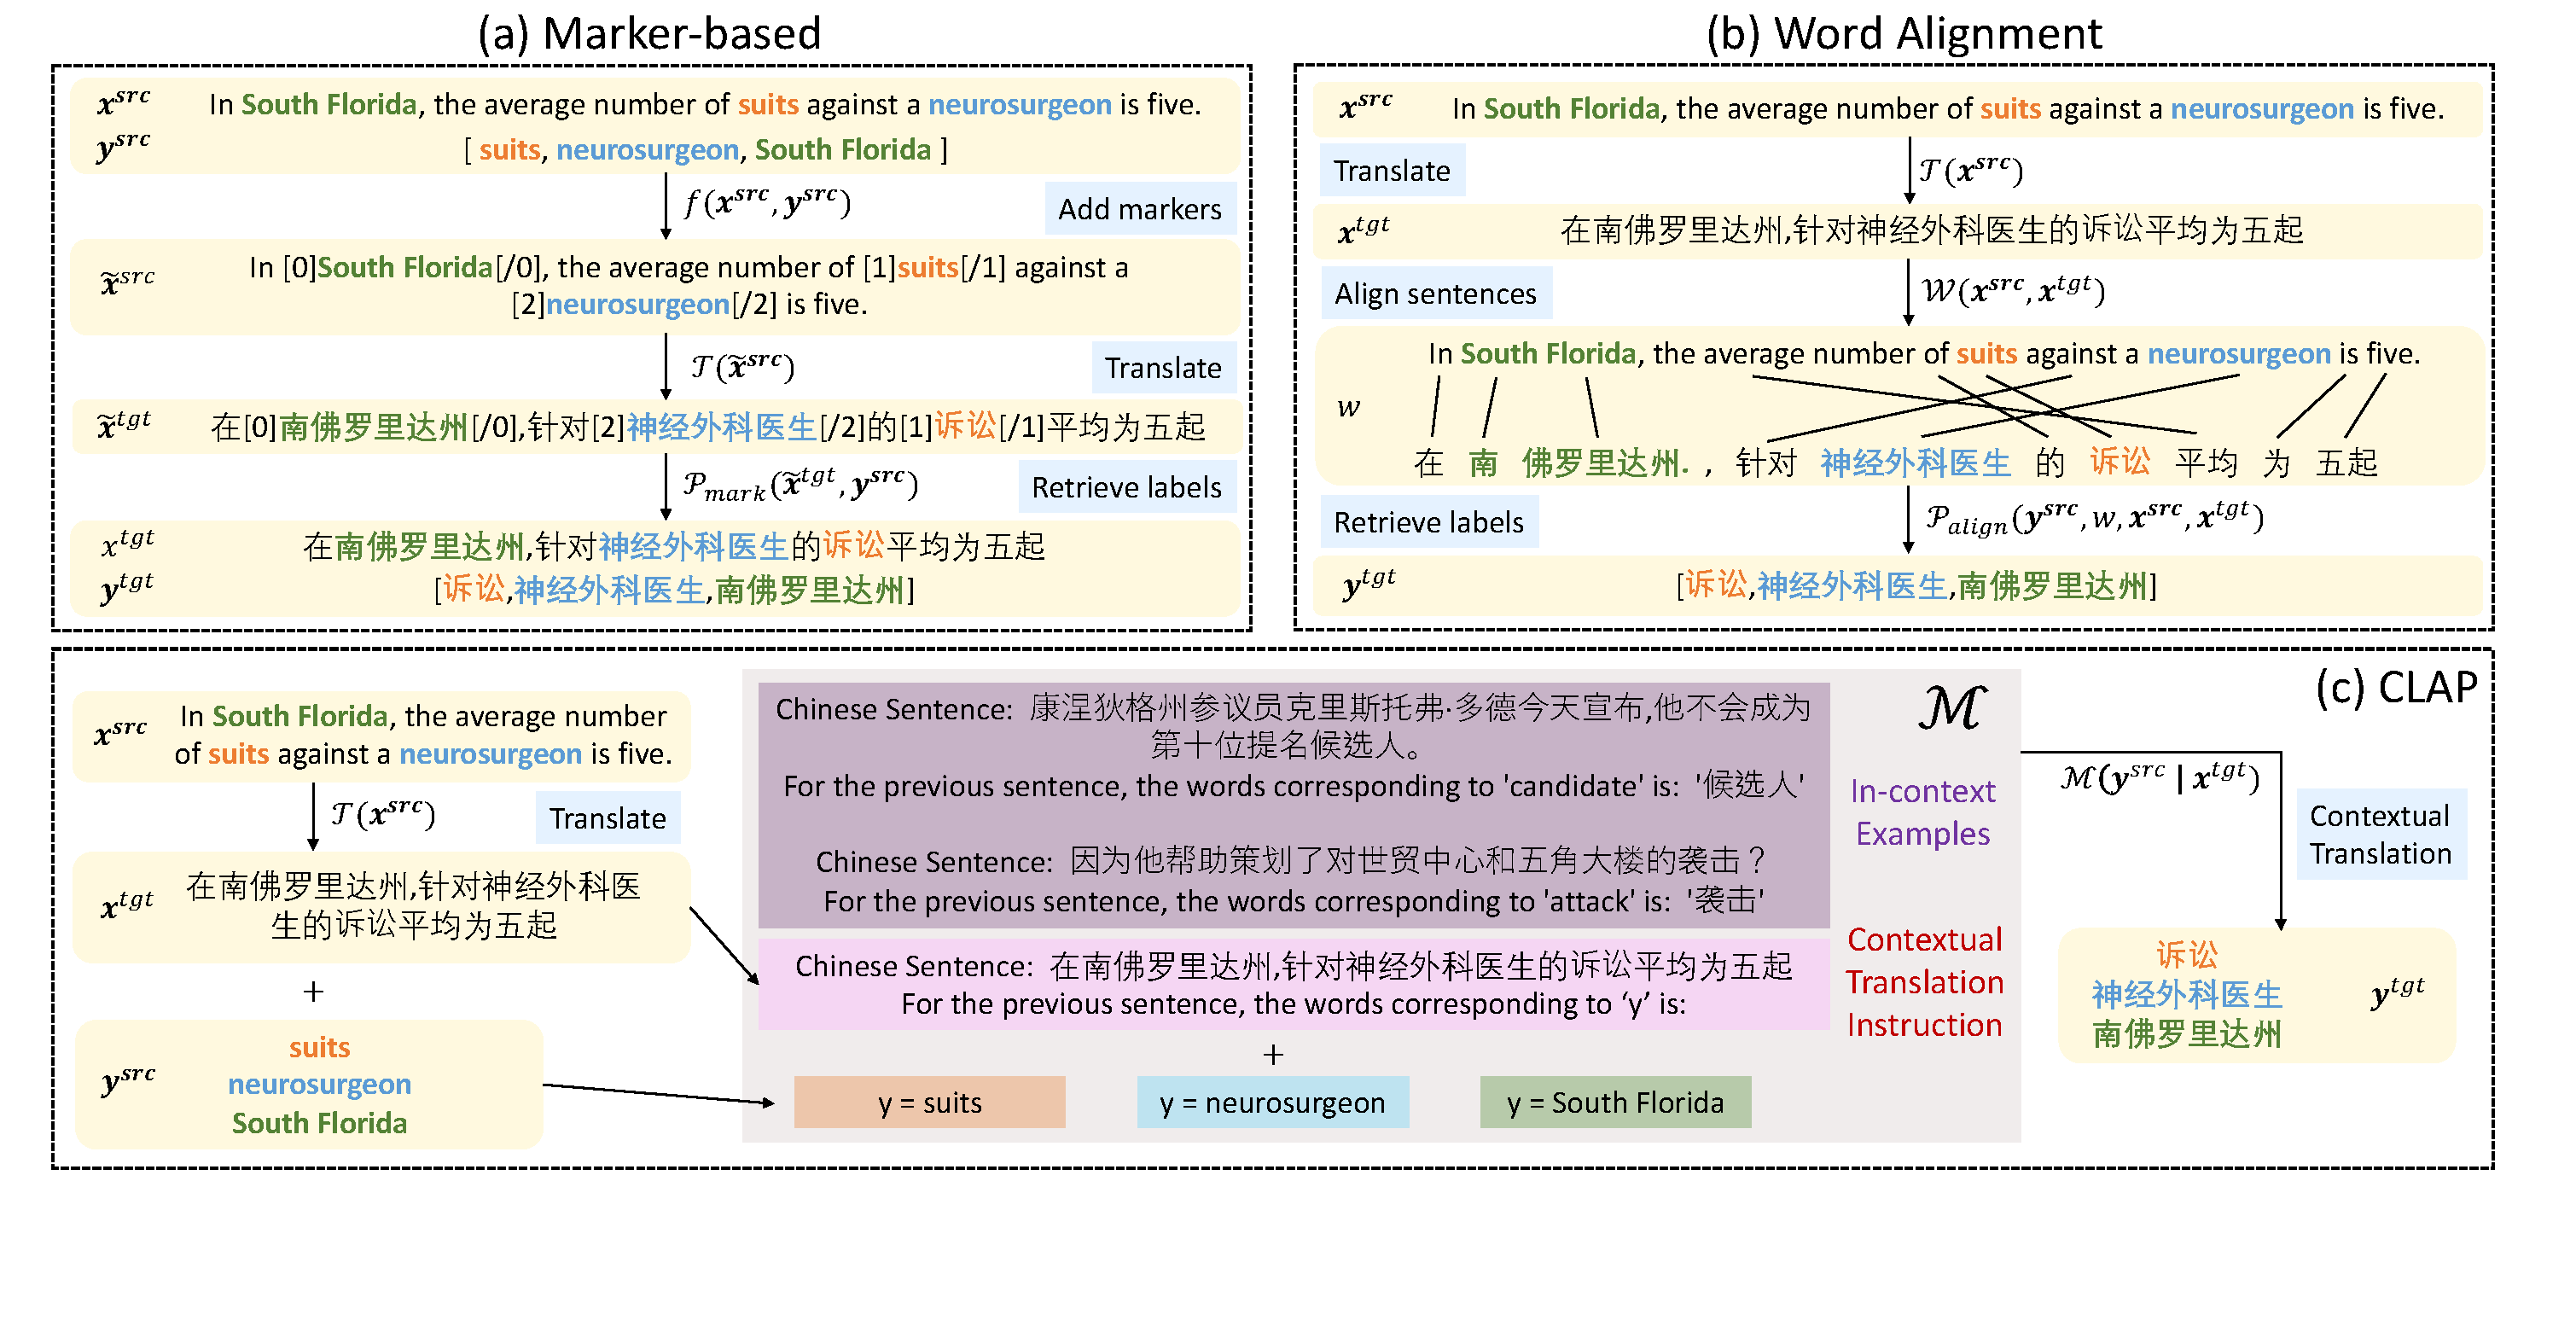
\includegraphics[height=0.4\textheight, clip, trim=0cm 10.7cm 24.5cm 1cm]{ClAP_marker_align.pdf}
    \caption{Marker-based methods. Illustration is from the CLAP paper.}
  \end{figure}
  \begin{columns}
    \begin{column}[t]{0.5\textwidth}
      \centering \textbf{CROP} \\
      \begin{flushleft}
        \textit{Markers}: \_\_SLOT1\_\_, ..., \_\_SLOTn\_\_ \\
        \textit{Idea}: save label for every slot
        \textit{Projection}: string matching between backtranslated and original enclosed in slots substrings
      \end{flushleft}
    \end{column}
    \begin{column}[t]{0.5\textwidth}
      \centering \textbf{EasyProject} \\
      \begin{flushleft}
        \textit{Markers}: [, ] \\
        \textit{Idea}: translate entities independently
        \textit{Projection}: fuzzy string matching between translated entities and
        enclosed in braces substrings
      \end{flushleft}
    \end{column}
  \end{columns}
\end{frame}

\begin{frame}
  \frametitle{Translation-based projection: T-Projection}
  \begin{figure}
    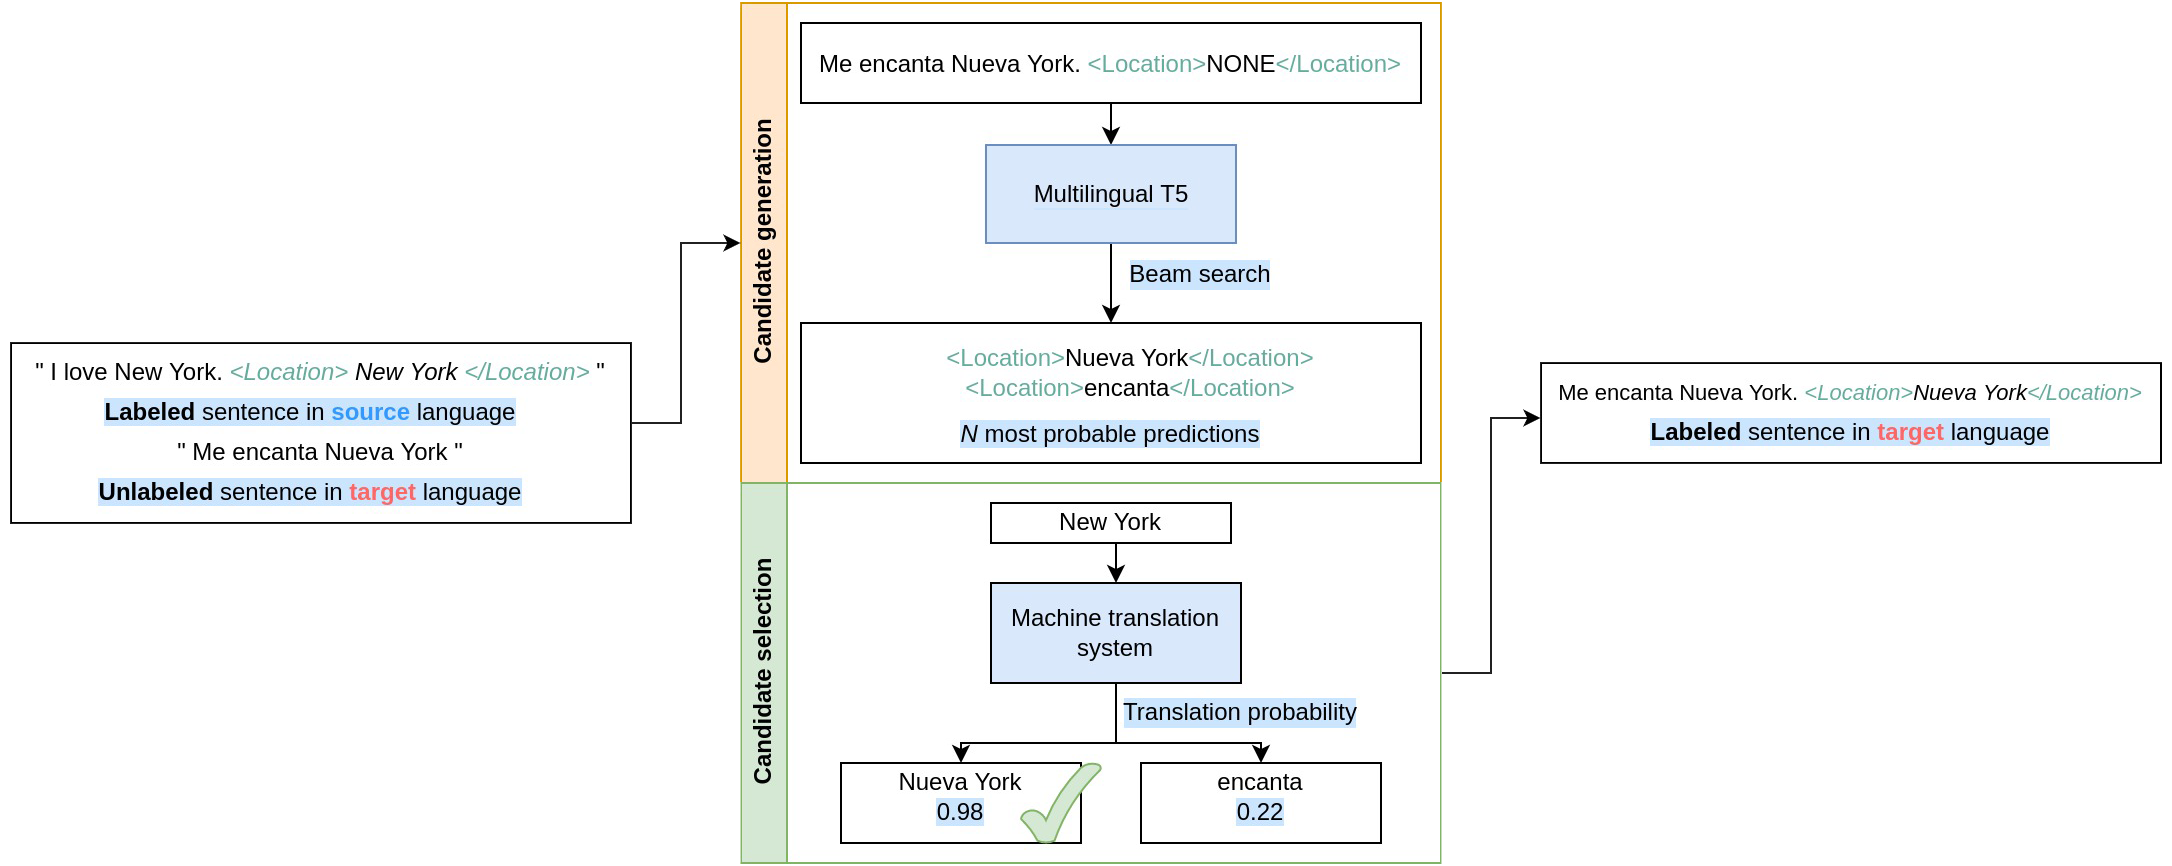
\includegraphics[width=\textwidth]{T-Projection.png}
    \caption{T-Projection. Illustration is from the original paper.}
  \end{figure}

  \begin{alertblock}{The closest related work}
    The idea is structurally similar to our method,
    but the projection step has not been formalized explicitly.
  \end{alertblock}
\end{frame}

\begin{frame}
  \frametitle{Translation-based projection: CLAP and CODEC}
  \begin{figure}
    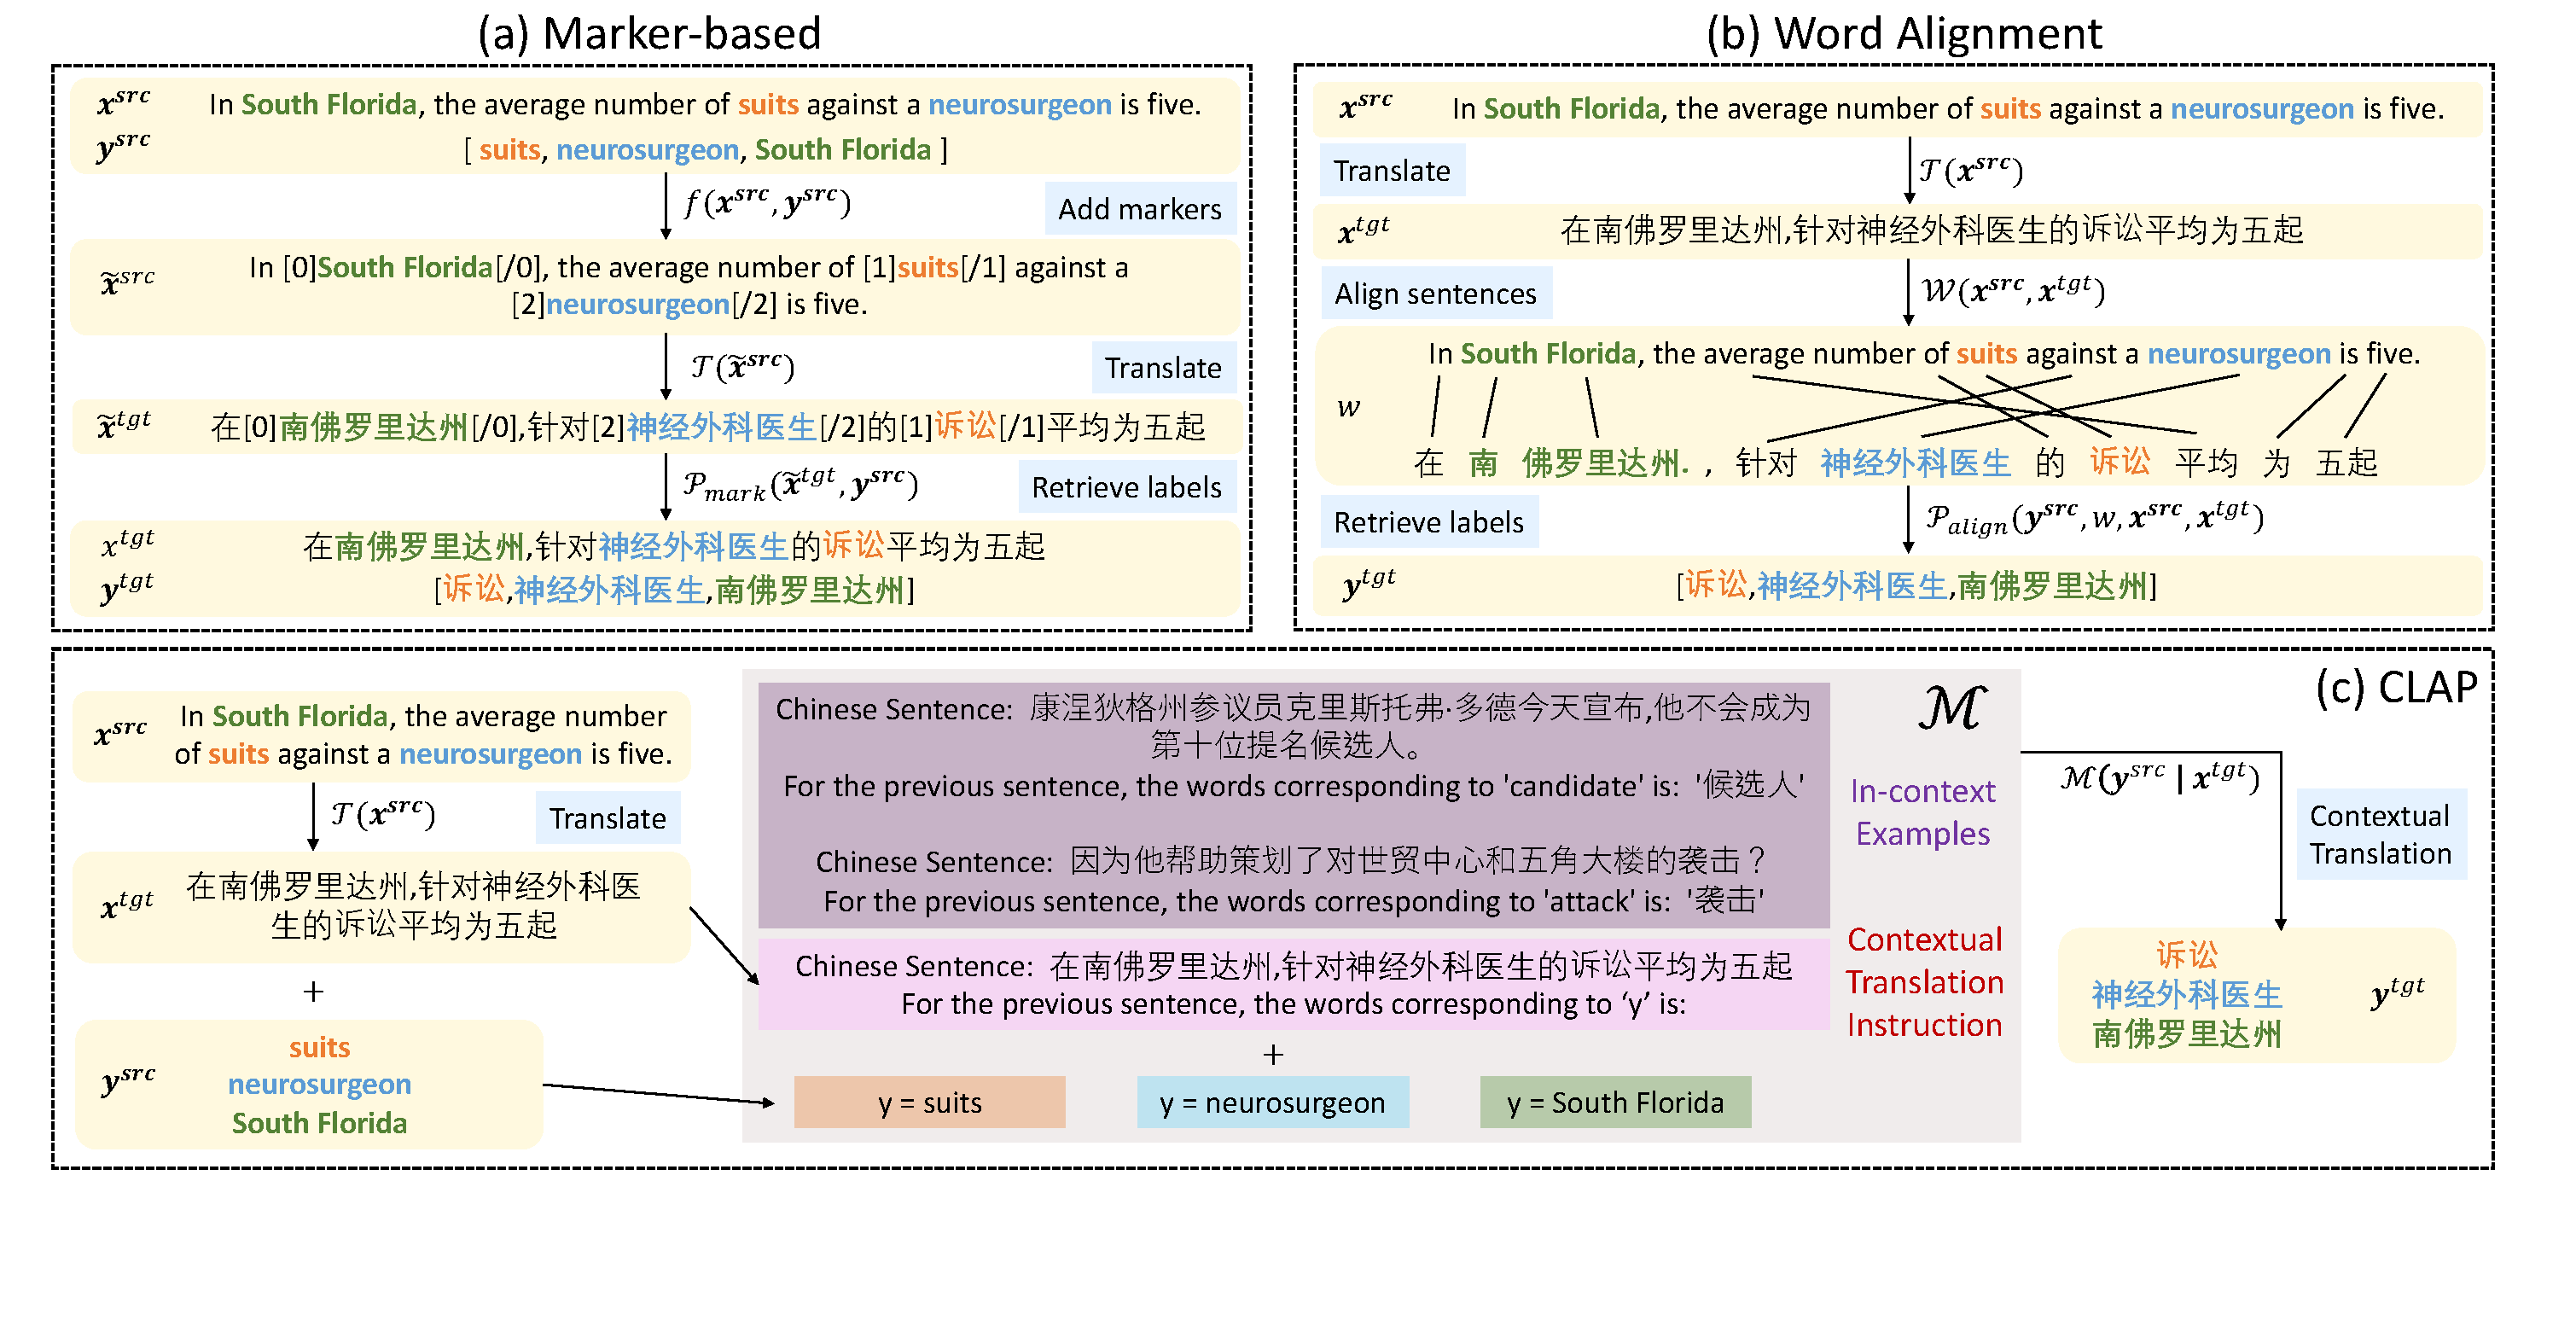
\includegraphics[width=0.95\textwidth, clip, trim=0cm 0cm 0cm 12.5cm]{ClAP_marker_align.pdf}
    \caption{Contextual Label Projection for Cross-Lingual Structured Prediction. Illustration is from the original paper.}
  \end{figure}
  \begin{figure}
    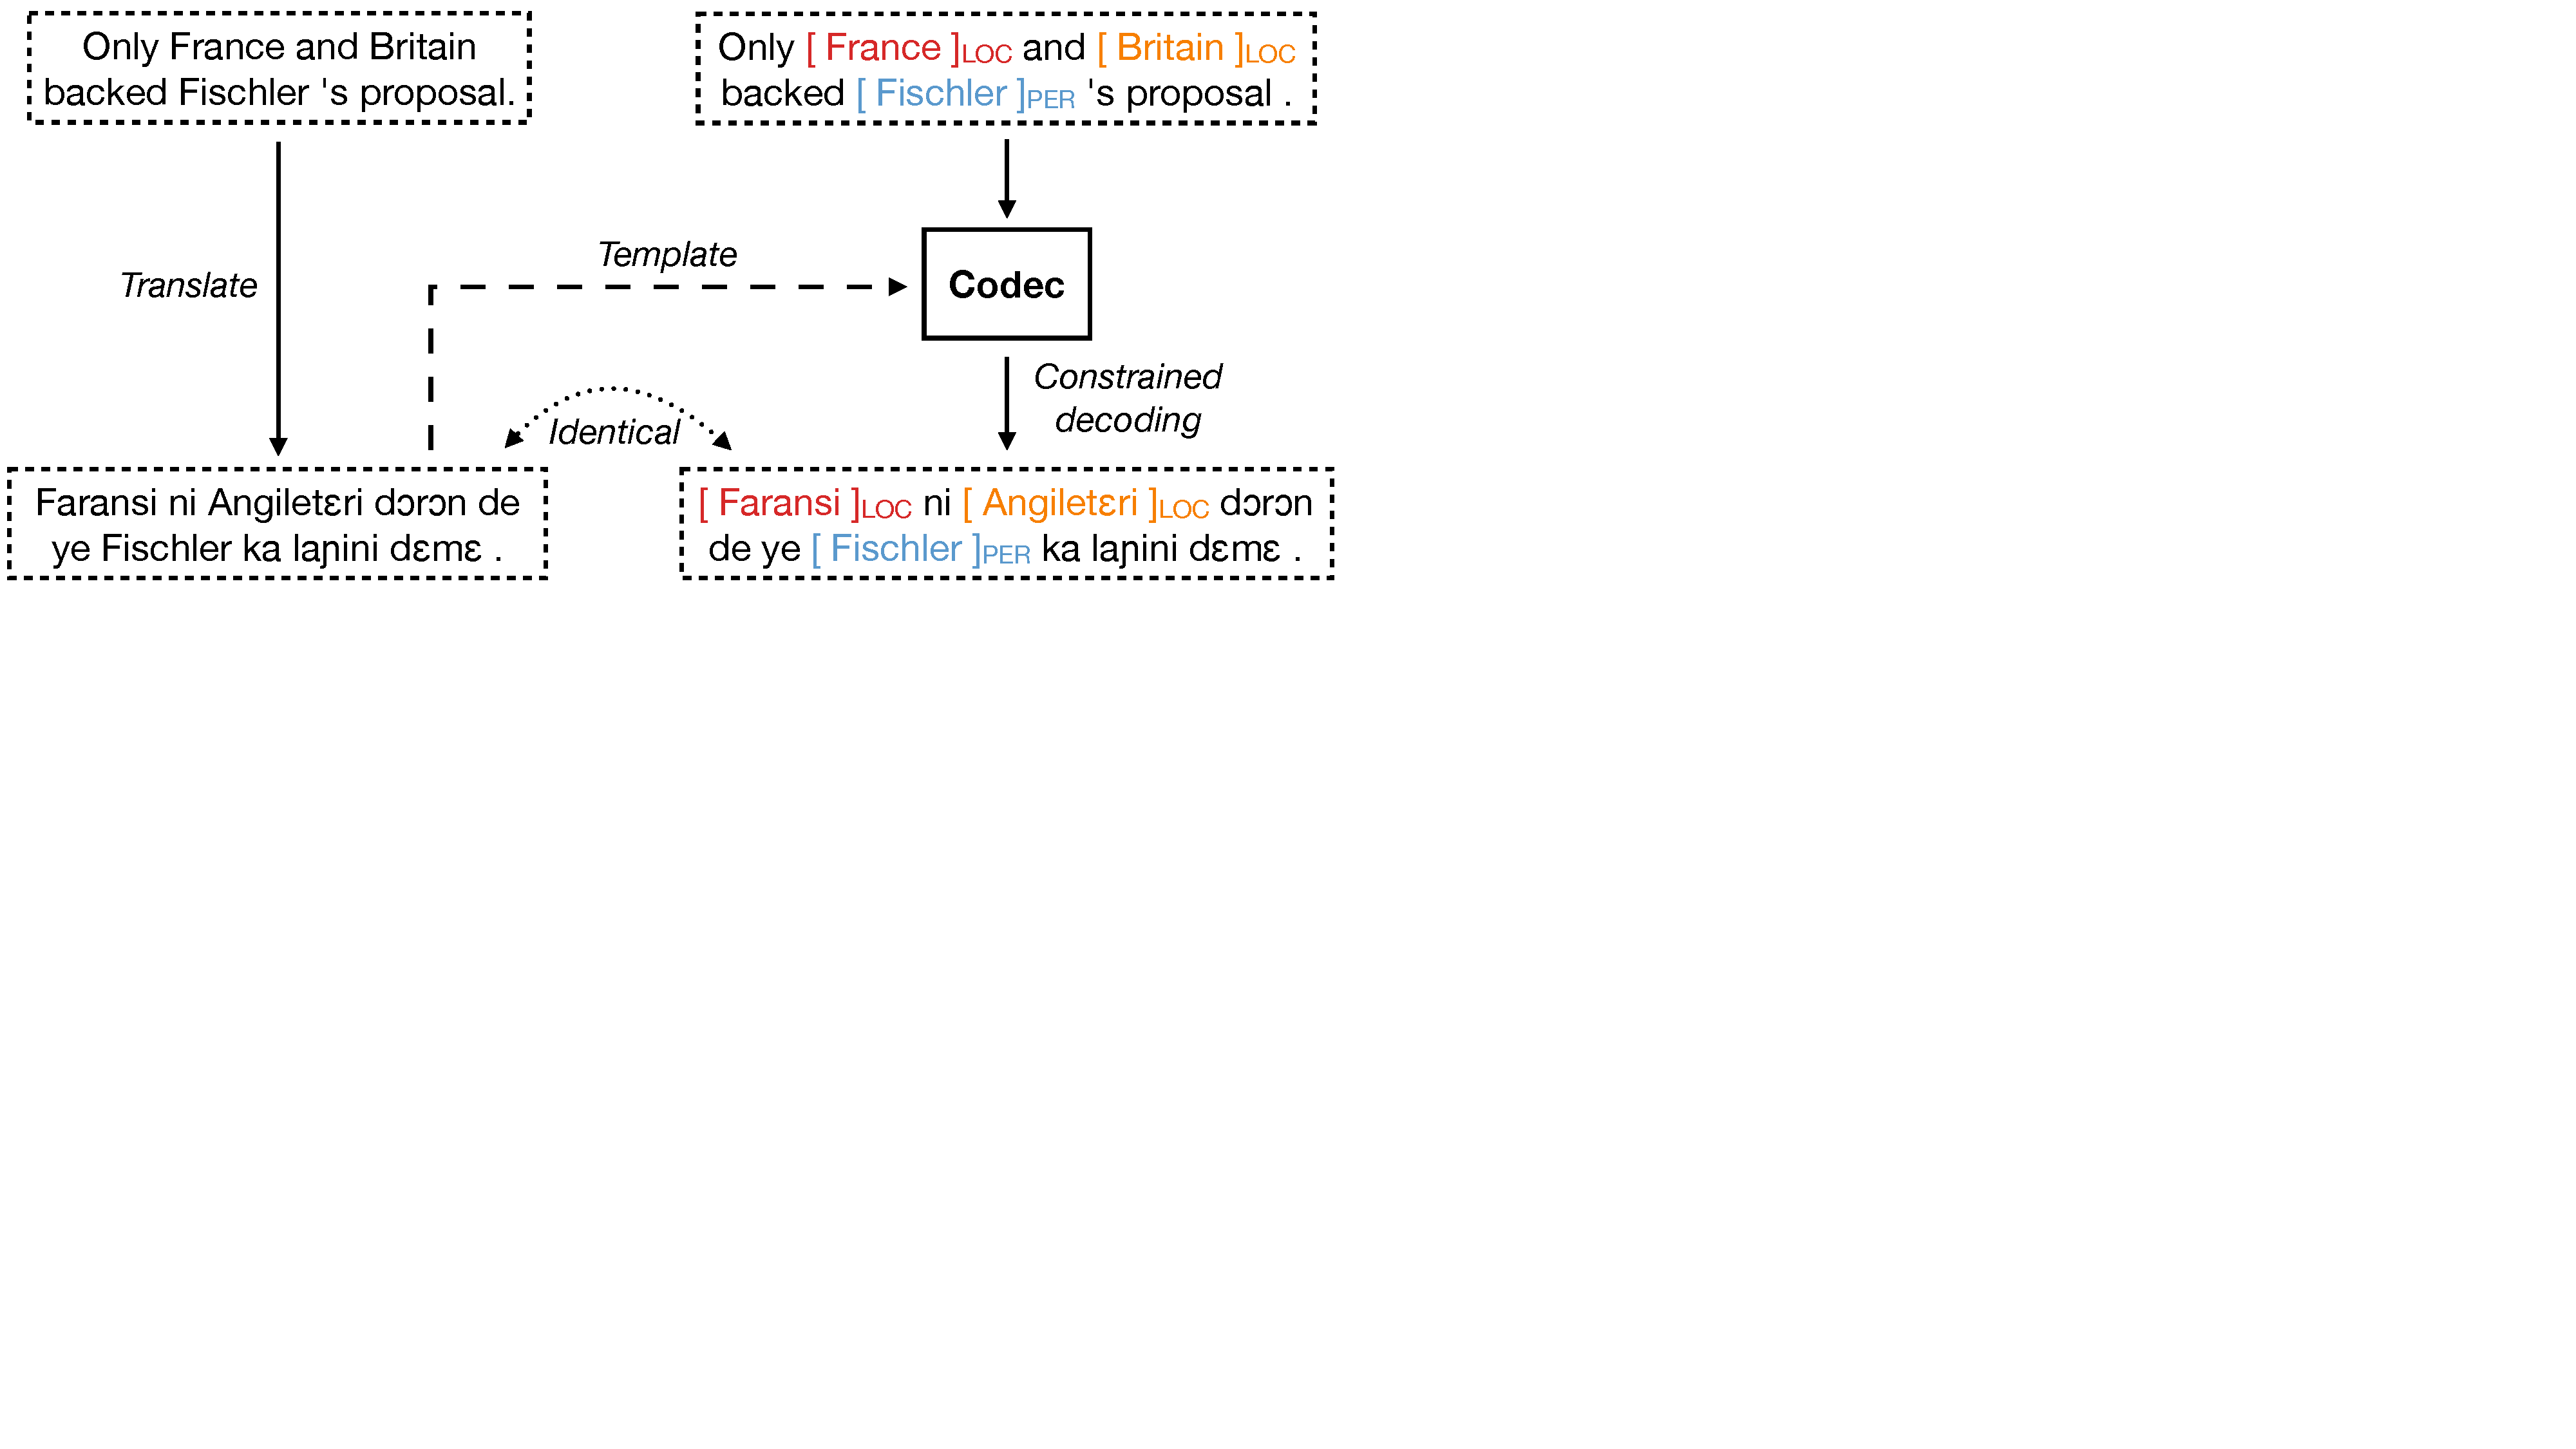
\includegraphics[height=0.3\textheight]{CODEC.pdf}
    \caption{Constrained Decoding for Cross-lingual Label Projection. Illustration is from the original paper.}
  \end{figure}
\end{frame}

\begin{frame}
  \frametitle{Model-based projection}

  \begin{block}{Idea}
    Use model to perform projection
  \end{block}

  TransFusion Decoder-only input/output format:
  \[
    [\text{GoLLIE Guidelines}, \text{src. sent}, \text{tgt. sent}, \text{Instructions}]
    \stackrel{}{\rightarrow}
    [\text{src. ent.}, \text{tgt. ent.}]
  \]

  TransFusion Encoder-only input format:\\
  \[
    \src{w_1},
    \src{w_2},
    \text{\textlangle PER\textrangle},
    \src{w_3},
    \text{\textlangle/PER\textrangle},
    \src{w_4},
    \text{\textlangle sep\textrangle},
    \tgt{w_1},
    \tgt{w_2},
    \tgt{w_3}
  \]

  \begin{alertblock}{Fundamental problem}
    TransFusion requires training, but if there are labelled parellel texts one can train a model in
    the target language directly
  \end{alertblock}
\end{frame}

\begin{frame}
  \frametitle{Word-to-word alignment-based projection}
  \begin{figure}
    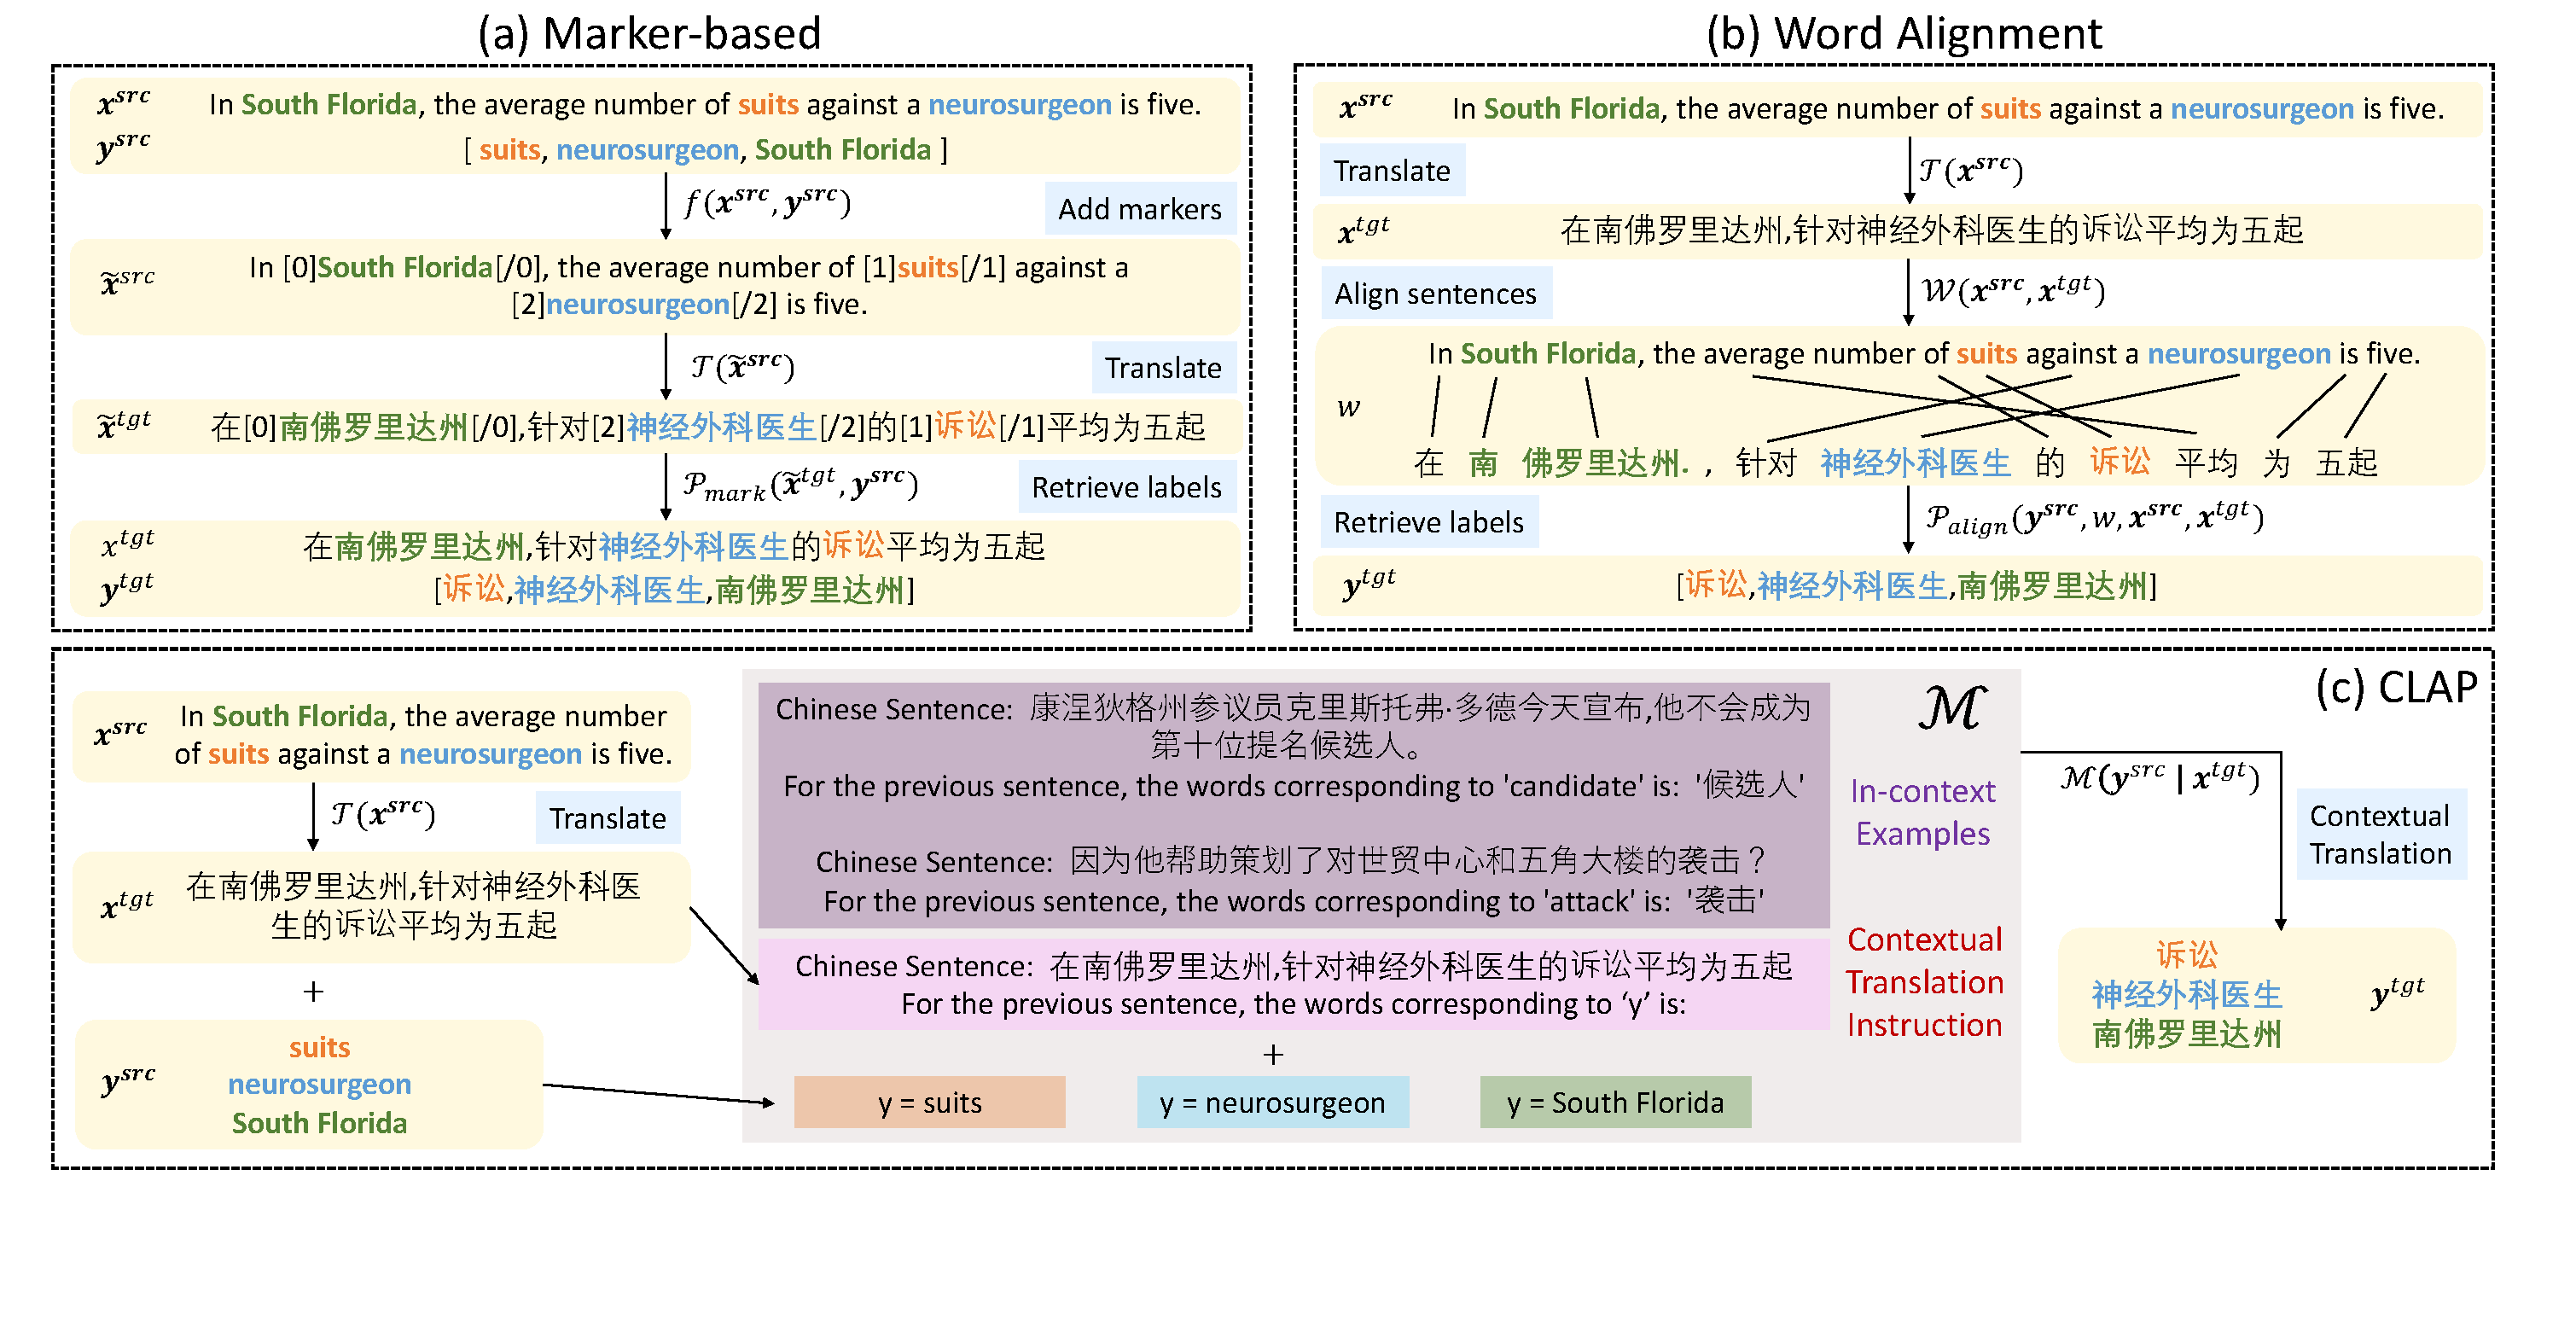
\includegraphics[height=0.4\textheight, clip, trim=24.5cm 10.7cm 0cm 1cm]{ClAP_marker_align.pdf}
    \caption{W2W alignment-based method. Illustration is from the CLAP paper.}
  \end{figure}

  \begin{flushleft}
    Issues and heuristics to handle them: \\
    \textit{Split annotations} \( \implies \) merge if only \( d \) non-aligned words are between \\
    \textit{Annotation collisions} \( \implies \) project only to the top-k by length ranges \\
    \textit{Incorrect alignments} \( \implies \) threshold by word length ratio
  \end{flushleft}
\end{frame}

\section{Methodology}

\begin{frame}
  \frametitle{Idea and requirements to the formalization}

  \begin{figure}
    \begin{tikzpicture}[node distance=-0.1,
        font=\footnotesize,
        % font=\fontsize{7pt}{10pt}\selectfont,
        every node/.style={text centered,
          text height=1.5ex,
        text depth=.25ex,},
        loc/.style={fill=orange!30, rounded rectangle, label={[anchor=center,font=\tiny\bfseries\sffamily]above:####1-LOC}},
        per/.style={fill=green!30, rounded rectangle, label={[anchor=center,font=\tiny\bfseries\sffamily]above:####1-PER}},
      cand/.style={fill=blue!30, rounded rectangle},]

      \node[per={B}, rounded rectangle east arc=none](Mark_src){Mark};
      \node[per={I}, rounded rectangle west arc=none, right=of Mark_src](Twain_src){Twain};
      \node[right=of Twain_src](was_src){was};
      \node[right=of was_src](born_src){born};
      \node[right=of born_src](in_src){in};
      \node[loc={B}, right=of in_src](Florida_src){Florida};

      \node[cand, rounded rectangle east arc=none, below=of Mark_src, yshift=-1.2cm](Mark_tgt){Mark};
      \node[cand, rounded rectangle west arc=none, right=of Mark_tgt](Twain_tgt){Twain};
      \node[right=of Twain_tgt](wurde_tgt){wurde};
      \node[right=of wurde_tgt](in_tgt){in};
      \node[cand, right=of in_tgt](Florida_tgt){Florida};
      \node[right=of Florida_tgt](geboren_tgt){geboren};

      \node[text=gray, font=\scriptsize, above=of born_src, yshift=0.2cm](source){Source labeled sentence};
      \node[text=gray, font=\scriptsize, below=of source, yshift=-2.45cm]{Original sentence with extracted candidates};

      \draw[->] (Mark_src.south east) -- node[left]{\(c_{11}\)} (Mark_tgt.north east);
      \draw[->] (Florida_src.south) -- node[right]{\(c_{22}\)} (Florida_tgt.north);
      \draw[->] (Mark_src.south east) -- node[above left, yshift=0.1cm]{\(c_{12}\)} (Florida_tgt.north);
      \draw[->] (Florida_src.south) -- node[above right, yshift=0.1cm]{\(c_{21}\)} (Mark_tgt.north east);
    \end{tikzpicture}
    \caption{Matching of extracted target candidates with source entities}
  \end{figure}

  Requirements:
  \begin{itemize}
    \item Projection onto overlapping candidates should not be possible.
    \item There is a limit on the number of projections from any source entity.
  \end{itemize}
\end{frame}

\begin{frame}
  \frametitle{Definitions}

  Let \( \src{s} = \left( \src{s_1}, \dots, \tgt{s_n} \right) \) and
  \( \tgt{s} = \left( \tgt{s_1}, \dots, \tgt{s_m} \right) \) be a source and target
  sentences respectively, \( L \) -- set of classes.
  \begin{block}{Source entity}
    The source entity \( \src{p} = (i_{\src{p}}, j_{\src{p}}, l_{\src{p}} ) \) is a continuous
    subrange of source words, where \( i_{\src{p}} \in \{ 1, \dots, n \} \) and
    \( j_{\src{p}} \in \{ 1, \dots, n \} \) are indices of
    the first and last word and \( l_{\src{p}} \in L \) is the class of the entity.
  \end{block}

  \begin{block}{Target candidate}
    The target candidate \( \tgt{p} = (i_{\tgt{p}}, j_{\tgt{p}}) \) is defined as a continuous
    subrange of target words.
  \end{block}

  \begin{block}{Relation of overlapping}
    \( \tgt{p_1} \cap \tgt{p_2} \neq \emptyset \Leftrightarrow
    ( i_{\tgt{p_1}} \leq j_{\tgt{p_2}} ) \land ( i_{\tgt{p_2}} \leq j_{\tgt{p_1}} ) \),
    i.e. the sets of words are not disjoint.
  \end{block}
\end{frame}

\begin{frame}
  \frametitle{Projection ILP problem}

  The projection problem is the following:
  \begin{align*}
    & \max\limits_x \sum\limits_{(\src{p}, \tgt{p}) \in S \times T} c_{\src{p}, \tgt{p}} x_{\src{p}, \tgt{p}} \\
    & \text{subject to}                                                                                                                      \\
    & \sum\limits_{\tgt{p} \in T} x_{\src{p}, \tgt{p}} \lessgtr n_{proj}
    \; \qquad \forall \src{p} \in S \\
    & x_{\src{p_1}, \tgt{p_1}} + x_{\src{p_2}, \tgt{p_2}} \leq 1
    \qquad \forall (\src{p_1}, \src{p_2}, \tgt{p_1}, \tgt{p_2}) \in \hat{\Pi}(S, T) \\
    & x_{\src{p}, \tgt{p}} \in \{ 0, 1 \}
    \; \;\qquad \qquad \forall (\src{p}, \tgt{p}) \in S \times T \notag
  \end{align*}
  where
  \begin{align*}
    \hat{\Pi}(S, T) = \Big\{ (\src{p_1}, \src{p_2}, \tgt{p_1}, \tgt{p_2}) \Big| \src{p_1}, \src{p_2} \in S, \tgt{p_1}, \tgt{p_2} \in T, \\
      \tgt{p_1} \cap \tgt{p_2} \neq \emptyset,
    (\src{p_1} \neq \src{p_2}) \lor (\tgt{p_1} \neq \tgt{p_2}) \Big\}
  \end{align*}
\end{frame}

\begin{frame}
  \frametitle{Reduction of the non-overlapping constraints}

  If it is impossible to project one or any two source entities onto overlapping
  candidates, then it is also impossible to project any number of source entities
  onto these candidates

  \begin{block}{Theorem}
    The set of non-overlapping constraints is satisfied if and only if
    the following sets of reduced constraints are satisfied:
    \begin{align*}
      & \sum\limits_{\src{p} \in S} (x_{\src{p}, \tgt{p_1}} + x_{\src{p}, \tgt{p_2}}) \leq 1
      \qquad \forall (\tgt{p_1}, \tgt{p_2}) \in \Pi(T) \\
      & \sum\limits_{\src{p} \in S} x_{\src{p}, \tgt{p}} \leq 1
      \qquad \forall \tgt{p} \in T \Big| \nexists \tgt{p_2} \in T: \tgt{p} \neq \tgt{p_2}, \tgt{p} \cap \tgt{p_2} \neq \emptyset                                             \\
      & \text{where} \\
      & \Pi(T) = \left\{ (\tgt{p_1}, \tgt{p_2}) \Big| \tgt{p_1}, \tgt{p_2} \in T,
        \quad \tgt{p_1} \cap \tgt{p_2} \neq \emptyset,
      \tgt{p_1} \neq \tgt{p_2} \right\}
    \end{align*}
  \end{block}

\end{frame}

\begin{frame}
  \frametitle{ILP problem with reduced number of constraints}
  The final form of the projection problem is
  \begin{align*}
    & \max\limits_x \sum\limits_{(\src{p}, \tgt{p}) \in S \times T} c_{\src{p}, \tgt{p}} x_{\src{p}, \tgt{p}}                                                                                                                       \\
    & \text{subject to}                                                                                                                                                                                                             \\
    & \sum\limits_{\tgt{p} \in T} x_{\src{p}, \tgt{p}} \lessgtr n_{proj}
    \qquad \forall \src{p} \in S                                                                                               \\
    & \sum\limits_{\src{p} \in S} (x_{\src{p}, \tgt{p_1}} + x_{\src{p}, \tgt{p_2}}) \leq 1
    \qquad \forall (\tgt{p_1}, \tgt{p_2}) \in \Pi(T)                                                                           \\
    & \sum\limits_{\src{p} \in S} x_{\src{p}, \tgt{p}} \leq 1
    \qquad \forall \tgt{p} \in T \Big| \nexists \tgt{p_2} \in T: \tgt{p} \neq \tgt{p_2}, \tgt{p} \cap \tgt{p_2} \neq \emptyset \\
    & x_{\src{p}, \tgt{p}} \in \{ 0, 1 \}
    \qquad \forall (\src{p}, \tgt{p}) \in S \times T
  \end{align*}
\end{frame}

\begin{frame}
  \frametitle{Candidate extraction}

  Let's consider the set of target candidates as all n-grams (composed of words from the target sentence).
  \begin{alertblock}{Problem: Number of candidates is too high}
    Limit the n-gram length to a fixed number.
  \end{alertblock}

  \begin{figure}
    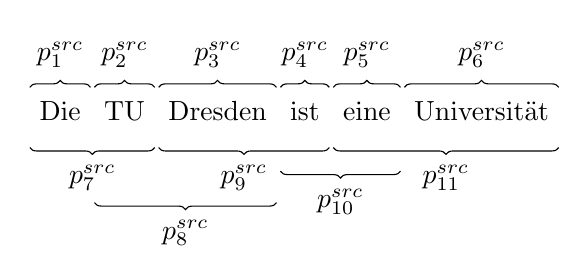
\begin{tikzpicture}[node distance=0.05,
        every node/.style={text centered,
          text height=2ex,
          text depth=.25ex,
      },]
      \node (1){Die};
      \node[right=of 1] (2){TU};
      \node[right=of 2] (3){Dresden};
      \node[right=of 3] (4){ist};
      \node[right=of 4] (5){eine};
      \node[right=of 5] (6){Universität};

      \draw[decoration={brace},decorate] (1.north west) -- node[above=5pt] {$\src{p_1}$} (1.north east);
      \draw[decoration={brace},decorate] (2.north west) -- node[above=5pt] {$\src{p_2}$} (2.north east);
      \draw[decoration={brace},decorate] (3.north west) -- node[above=5pt] {$\src{p_3}$} (3.north east);
      \draw[decoration={brace},decorate] (4.north west) -- node[above=5pt] {$\src{p_4}$} (4.north east);
      \draw[decoration={brace},decorate] (5.north west) -- node[above=5pt] {$\src{p_5}$} (5.north east);
      \draw[decoration={brace},decorate] (6.north west) -- node[above=5pt] {$\src{p_6}$} (6.north east);

      % \node (anchor_p8) at (3.south east)++(0, 1) {};

      \draw[decoration={brace,mirror,raise=5pt},decorate] (1.south west) -- node[below=6pt] {$\src{p_7}$} (2.south east);
      \draw[decoration={brace,mirror,raise=5pt},decorate] (2.south west)++(0,-0.7) -- node[below=6pt] {$\src{p_8}$} ($(3.south east)+(0,-0.7)$);
      \draw[decoration={brace,mirror,raise=5pt},decorate] (3.south west) -- node[below=6pt] {$\src{p_9}$} (4.south east);
      \draw[decoration={brace,mirror,raise=5pt},decorate] (4.south west)++(0,-0.3) -- node[below=6pt] {$\src{p_{10}}$} ($(5.south east)+(0,-0.3)$);
      \draw[decoration={brace,mirror,raise=5pt},decorate] (5.south west) -- node[below=6pt] {$\src{p_{11}}$} (6.south east);
    \end{tikzpicture}
    \caption{An example of a target candidate extraction algorithm with an n-gram length limit of 2 words}
  \end{figure}
  % \begin{exampleblock}{Example}
  %   Targert sentence: \texttt{Die TU Dresden ist eine Universität}
  %   Set of target candidates \( T = \{ (0, 1), () \} \)
  % \end{exampleblock}

\end{frame}

\begin{frame}
  \frametitle{Word-to-word alignment-based matching score}

  Let \( a_{kl} \) be binary variable denoted if \( k \)-th source word aligned to \( l \) target word,
  then the word-to-word alignment-based mathcing score is the following:

  \begin{equation*}
    c_{\src{p}, \tgt{p}}^{align} =
    \frac{\sum\limits_{k=i_{\src{p}}}^{j_{\src{p}}} \sum\limits_{l=i_{\tgt{p}}}^{j_{\tgt{p}}} a_{kl}}
    {(j_{\src{p}} - i_{\src{p}}) + (j_{\tgt{p}} - i_{\tgt{p}})}
  \end{equation*}

  \vspace*{0.2cm}
  \begin{columns}
    \begin{column}[t]{.5\textwidth}
      \centering \textbf{Pros:}
      \begin{itemize}
        \item Alignments \( \rightarrow \) quanitive score
        \item Allow to reduce set of target candidates
      \end{itemize}
    \end{column}
    \begin{column}[t]{.5\textwidth}
      \centering \textbf{Cons:}
      \begin{itemize}
        \item "Merging" heuristic is not always preserved
      \end{itemize}
    \end{column}
  \end{columns}
\end{frame}

\begin{frame}
  \frametitle{Reduction of the set of candidates}
\end{frame}

\begin{frame}
  \frametitle{NER model-based matching score}
  Let \( p_{k,l} \) be the probability predicted by a NER model that the \( k \)-th
  target word has a label \( l \in L \). Let \( \mathcal{B} \) and \( \mathcal{I} \) be
  mappings that return the indices of B- and I- labels in the model output matrix.
  Then the NER-based score is defined as follows:
  \begin{equation*}
    c_{\src{p}, \tgt{p}}^{ner} = \alpha^{(j_{\tgt{p}} - i_{\tgt{p}}) - 1}
    \frac{
      p_{i_{\tgt{p}}, \mathcal{B}[l_{\src{p}}]} +
      \sum\limits_{k = i_{\tgt{p}} + 1}^{j_{\tgt{p}}} p_{k, \mathcal{I}[l_{\src{p}}]}
    }
    {j_{\tgt{p}} - i_{\tgt{p}}}
  \end{equation*}

  \vspace*{0.2cm}
  \begin{columns}
    \begin{column}[t]{.5\textwidth}
      \centering \textbf{Pros:}
      \begin{itemize}
        \item Projection \( \implies \) can correct missed/wrongly predicted by a
          NER model entities
      \end{itemize}
    \end{column}
    \begin{column}[t]{.5\textwidth}
      \centering \textbf{Cons:}
      \begin{itemize}
        \item Projection \( \implies \) depends on quality of source NER labelling
        \item Scores are identical for all source entities sharing the same class
        \item Overconfidence of NER models
      \end{itemize}
    \end{column}
  \end{columns}
\end{frame}

\begin{frame}
  \frametitle{NER model-based matching score: alpha parameter}
  Let \( s \) be a source entity with label \texttt{PER}.
  And the model output is the following:

  \begin{figure}[ht]
    \centering
    \begin{tikzpicture}[node distance=-0.1,
        every node/.style={text centered,
          text height=2ex,
          text depth=.25ex,
        },
        loc/.style={fill=orange!30, rounded rectangle, label={[anchor=center,font=\tiny\bfseries\sffamily]above:####1}},
        per/.style={fill=green!30, rounded rectangle, label={[anchor=center,font=\tiny\bfseries\sffamily]above:####1}},
        O/.style={rounded rectangle, label={[anchor=center,font=\tiny\bfseries\sffamily]above:O}}
      ]

      \node[per={0.9}, rounded rectangle east arc=none](Mark_tgt){Mark};
      \node[per={0.8}, rounded rectangle west arc=none, right=of Mark_tgt](Twain_tgt){Twain};
      \node[right=of Twain_tgt](wurde_tgt){wurde};
      \node[right=of wurde_tgt](in_tgt){in};
      \node[loc={0.95}, right=of in_tgt](Florida_tgt){Florida};
      \node[right=of Florida_tgt](geboren_tgt){geboren};
    \end{tikzpicture}
    % \caption{Example of missaligned prediction when }
  \end{figure}

  If \( \alpha = 1 \), then the output of the projection step will be
  misaligned with the output of the NER model:
  \[
    c^{ner}_{s, "Mark"} = 0.9 \qquad c^{ner}_{s, "Mark Twain"} = 0.85
  \]

  \begin{block}{Estimation of \( \alpha \)}
    Let \( M = \frac{1}{2|L| + 1} \). Then, if
    \(\alpha > 1 + \frac{1 - M}{1 + M}\),
    the predictions of the projection step and the NER model are aligned.
  \end{block}

\end{frame}

\begin{frame}
  \frametitle{Translation-based matching score}
  The idea is to compute how likely a source entity is translated into a target
  candidate. To accomplish this, we use the NMTScore (denoted as the \( sim \) function):
  \begin{equation*}
    c_{\src{p}, \tgt{p}}^{nmt} =
    sim \left(\src{w}[i_{\src{p}} : j_{\src{p}}],
    \tgt{w}[i_{\tgt{p}} : j_{\tgt{p}}] \right)
  \end{equation*}

  \vspace*{0.2cm}
  \begin{columns}
    \begin{column}[t]{.5\textwidth}
      \centering \textbf{Pros:}
      \begin{itemize}
        \item Interpretability
      \end{itemize}
    \end{column}
    \begin{column}[t]{.5\textwidth}
      \centering \textbf{Cons:}
      \begin{itemize}
        \item Translation without context
        \item Slower then other scores
      \end{itemize}
    \end{column}
  \end{columns}
\end{frame}

\begin{frame}
  \frametitle{Fused matching score}
  Since all matching score are just real numbers we can compute a weighted sum of them,
  i.e. combine different projection strategies together:
  \begin{equation*}
    c_{\src{p}, \tgt{p}}^{fused} =
    \lambda_{align} c_{\src{p}, \tgt{p}}^{align} +
    \lambda_{ner} c_{\src{p}, \tgt{p}}^{ner} +
    \lambda_{nmt} c_{\src{p}, \tgt{p}}^{nmt}
  \end{equation*}
  where \( \lambda_{align} \geq 0, \lambda_{ner} \geq 0, \lambda_{nmt} \geq 0 \in \mathbb{R}\).

  \vspace*{0.3cm}
  Then, NER-based score can be used to evaluate only spans without labels:
  \begin{equation*}
    c_{\src{p}, \tgt{p}}^{ner} = \alpha^{(j_{\tgt{p}} - i_{\tgt{p}}) - 1}
    \max\limits_{l \in L}
    \frac{
      p_{i_{\tgt{p}}, B[l]} +
      \sum\limits_{k = i_{\tgt{p}} + 1}^{j_{\tgt{p}}} p_{k, I[l]}
    }
    {j_{\tgt{p}} - i_{\tgt{p}}}
  \end{equation*}
\end{frame}

% \begin{frame}
%   \frametitle{Example of the ILP problem}
% \end{frame}

\begin{frame}
  \frametitle{Complexity}

  \begin{columns}
    \begin{column}{.5\textwidth}
      Current results:
      \begin{itemize}
        \item MaxIS is reducible to the generalized problem with target candidates
          beyond intervals \( \implies \) NP-Hard
        \item The ILP problem without constraint on number of
          projections reduces to MaxWIS on \textbf{interval graphs}  \( \implies \) can be solved in polynomial time
      \end{itemize}

      \begin{alertblock}{}
        Complexity of the original projection problem remains an open question.
      \end{alertblock}
    \end{column}
    \begin{column}{.5\textwidth}
      \begin{figure}[ht]
        \centering
        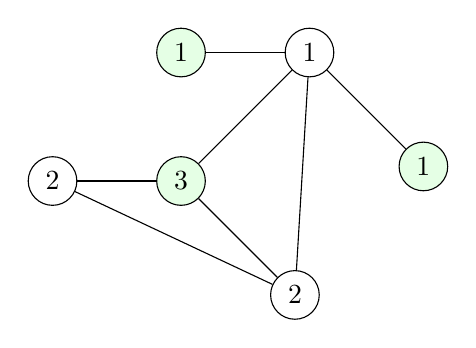
\begin{tikzpicture}[every node/.style = {draw, circle}]
          \node[fill=green!10] (1) {1};
          \node[right=of 1] (2) {1};
          \node[below right=of 2, fill=green!10] (3) {1};
          \node[below=of 1, fill=green!10] (4) {3};
          \node[left=of 4] (5) {2};
          \node[below right=of 4] (6) {2};

          \graph{
            (1) -- (2) -- (4) -- (6) -- (5) -- (4),
            (6) -- (2) -- (3)
          };
        \end{tikzpicture}
        \caption{Maximum weight independent set problem (MaxWIS). Vertices that form an optimal solution are colored in green}
        \label{fig:maxwis}
      \end{figure}
    \end{column}
  \end{columns}
\end{frame}

\begin{frame}
  \frametitle{Reduction to the MaxWIS problem}
  \begin{columns}
    \begin{column}[t]{.5\textwidth}
      \centering\textbf{Simplified projection problem}
      \begin{align*}
        & \max\limits_x \sum\limits_{(\src{p}, \tgt{p}) \in S \times T} c_{\src{p}, \tgt{p}} x_{\src{p}, \tgt{p}}                                             \\
        & \text{subject to}                                                                                                                                   \\
        & x_{\src{p_1}, \tgt{p_1}} + x_{\src{p_2}, \tgt{p_2}} \leq 1\\
        & x_{\src{p}, \tgt{p}} \in \{ 0, 1 \}
      \end{align*}
    \end{column}
    \begin{column}[t]{.5\textwidth}
      \centering\textbf{MaxWIS problem}
      \begin{align*}
        & \max \sum\limits_{v \in V} w_v x_v                               \\
        & \text{subject to} \\
        & x_u + x_v \leq 1               \qquad \forall \{u, v\} \in E \\
        & x_v \in \{0, 1\}
      \end{align*}
    \end{column}
  \end{columns}

  \centering\textbf{Reduction}
  \[
    w_v = \max\limits_{s \in S} c_{s, t_v} \qquad s^*_v = \argmax\limits_{s \in S} x_{s, t_v}
  \]
  \[
    x_v = 1 \implies
    \begin{cases}
      x_{s^*, t_v} = 1 \\
      x_{s, t_v} = 0 \quad \forall s \in S \setminus \{ s^* \}
    \end{cases}
  \]
  \[
    \{ v, u \} \in E \Leftrightarrow t_u \cap t_v \neq \emptyset
  \]
\end{frame}

\begin{frame}
  \frametitle{Reduction to the MaxWIS problem}

  \begin{columns}

    \begin{column}[t]{.5\textwidth}
      \begin{figure}
        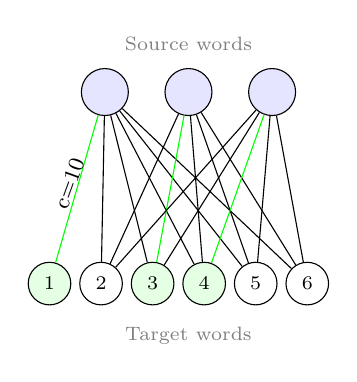
\begin{tikzpicture}[
            node distance=0.1,
            realstate/.style = {draw, circle, font=\scriptsize},
            dummystate/.style = {draw, circle, minimum width=4, inner sep=6, fill=blue!10}
          ]
          \node[dummystate] (src_1) {};
          \node[right=of src_1, xshift=10, dummystate] (src_2) {};
          \node[right=of src_2, xshift=10, dummystate] (src_3) {};

          \node[below=of src_1, fill=green!10, xshift=-20, yshift=-1.75cm, realstate] (1) {1};
          \node[right=of 1, realstate] (2) {2};
          \node[right=of 2, fill=green!10, realstate] (3) {3};
          \node[right=of 3, fill=green!10, realstate] (4) {4};
          \node[right=of 4, realstate] (5) {5};
          \node[right=of 5, realstate] (6) {6};

          \node[above=of src_2, text=gray, font=\scriptsize] {Source words};
          \node[below=of src_2, yshift=-70, text=gray, font=\scriptsize] {Target words};

          \draw[green] (src_1) -- node[above, xshift=3, rotate=70, black, font=\footnotesize]{c=10} (1);
          \draw (src_1) -- (2);
          \draw (src_1) -- (3);
          \draw (src_1) -- (4);
          \draw (src_1) -- (5);
          \draw (src_1) -- (6);
          \draw (src_2) -- (2);
          \draw[green] (src_2) -- (3);
          \draw (src_2) -- (4);
          \draw (src_2) -- (5);
          \draw (src_2) -- (6);
          \draw (src_3) -- (2);
          \draw (src_3) -- (3);
          \draw[green] (src_3) -- (4);
          \draw (src_3) -- (5);
          \draw (src_3) -- (6);
        \end{tikzpicture}
        \caption{The simplified projeciton problem, maximum weight edges are colored in green}
      \end{figure}
    \end{column}
    \begin{column}[t]{.5\textwidth}
      \begin{figure}
        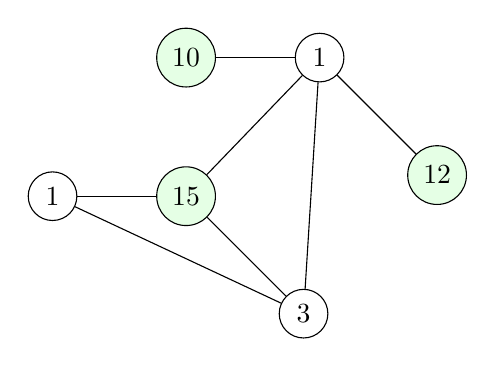
\begin{tikzpicture}[every node/.style = {draw, circle}]
          \node[fill=green!10] (1) {10};
          \node[right=of 1] (2) {1};
          \node[below right=of 2, fill=green!10] (3) {12};
          \node[below=of 1, fill=green!10] (4) {15};
          \node[left=of 4] (5) {1};
          \node[below right=of 4] (6) {3};

          \graph{
            (1) -- (2) -- (4) -- (6) -- (5) -- (4),
            (6) -- (2) -- (3)
          };
        \end{tikzpicture}
        \caption{Induced maximum weight independent set problem on an interval graph}
      \end{figure}
    \end{column}
  \end{columns}

\end{frame}

\tikzstyle{startstop} = [rectangle, rounded corners, text width=2cm, minimum height=1cm,text centered, draw=black, fill=red!30]
\tikzstyle{process} = [rectangle, text width=2.2cm, minimum height=1.5cm, text centered, draw=black, fill=orange!30, font={\small}]
\tikzstyle{decision} = [diamond, text width=1.2cm, minimum height=1cm, text centered, draw=black, fill=green!30, font={\small}]
\tikzstyle{arrow} = [thick,->,>=stealth]

\begin{frame}
  \frametitle{Approximate algorithm}
  \begin{figure}
    \begin{tikzpicture}[node distance=1]
      \node (start) [startstop] {Input: ILP Problem};
      \node (dec1) [decision, below=of start] {\( \exists s, t \Big| \) \linebreak \( c_{s, t} > 0 \)};
      \node (stop) [startstop, left=of dec1] {Output:  projections};
      \node (proc1) [process, below=of stop, yshift=-25] {Take maximum score projecion};
      \node (proc2) [process, below=of dec1, yshift=-2] {Remove all overlapping candidates};
      \node (proc3) [process, right=of proc2, dashed, fill=orange!15] {Remove source entities that reach limit};

      \node[fill=orange!30, draw=black] at (proc3.north east) {\( <, \leq, = \)};

      \draw [arrow] (start) -- (dec1);
      \draw [arrow] (dec1) -- node[anchor=south]{false} (stop);
      \draw [arrow] (dec1) |- node[anchor=south east]{true} (0, -4.7) -| (proc1);
      \draw [arrow] (proc1) -- (proc2);
      \draw [arrow] (proc2) -- (proc3);
      \draw [arrow] (proc3) |- (dec1);
    \end{tikzpicture}
  \end{figure}
\end{frame}

\begin{frame}
  \frametitle{Example of approximate algorithm failure}

  Consider the ILP problem with \( n_{proj} = 2 \) and the \( \leq \)
  type of constraints.
  Let \( T = \{ \tgt{p_1} = (1, 2), \tgt{p_2} = (2, 3), \tgt{p_3} = (3, 5) \} \)
  and \( S = \{ \src{p} \} \), and let the matching scores be as follows:
  \begin{table}
    \begin{tabular}{cccc}
      & $ \tgt{p_1} $ & $ \tgt{p_2} $  & $\tgt{p_3}$ \\
      \toprule
      $ \src{p} $ & 0.2 & 0.3 & 0.2 \\
    \end{tabular}
  \end{table}
  Note, that \( \tgt{p_1} \cap \tgt{p_2} \neq \emptyset \) and \( \tgt{p_2} \cap \tgt{p_3} \neq \emptyset \), but \( \tgt{p_2} \cap \tgt{p_3} = \emptyset \)
  \vspace*{0.2cm}
  \begin{columns}
    \hspace*{0.1cm}
    \begin{column}[t]{0.5\textwidth}
      \textbf{The output of the Algorithm:} \\
      \( x_{\src{p}, \tgt{p_1}} = 0 \) \\
      \( x_{\src{p}, \tgt{p_2}} = 1 \) \\
      \( x_{\src{p}, \tgt{p_3}} = 0 \) \\
      \vspace*{0.2cm}
      Objective value: \( 0.3 \)
    \end{column}
    \begin{column}[t]{0.5\textwidth}
      \textbf{Optimal solution:} \\
      \( x_{\src{p}, \tgt{p_1}} = 1 \) \\
      \( x_{\src{p}, \tgt{p_2}} = 0 \) \\
      \( x_{\src{p}, \tgt{p_3}} = 1 \) \\
      \vspace*{0.2cm}
      Objective value: \( 0.4 \)
    \end{column}
  \end{columns}
  % \[
  %   c_{\src{p}, \tgt{p_1}} = 0.2 \qquad
  %   c_{\src{p}, \tgt{p_2}} = 0.3 \qquad
  %   c_{\src{p}, \tgt{p_3}} = 0.2
  % \]
\end{frame}

\section{Evaluation}

\begin{frame}
  \frametitle{Experiments setup}

  \begin{itemize}
    \item Intrinsic evaluation
    \item Translation and NER models are shared between experiments
    \item Translation model: NLLB-200
    \item NER model: MDeBERTa-v3-base finetuned on the English split of the CONLL-2003
    \item Aligner: non-finetuned AWeSOME with default parameters
    \item Maximum candidate length: 10 words
    \item Exact ILP solver: GUROBI
  \end{itemize}
\end{frame}

\begin{frame}
  \frametitle{Europarl-NER: Heuristics}

  \begin{table}[ht]
    \centering
    \scalebox{0.75}{
      \begin{tabular}{llllrrr}
  \toprule
  &  &  & tgt\_lang & de & es & it \\
  d & k & only\_i & thr &  &  &  \\
  \midrule
  \multirow[t]{8}{*}{0} & \multirow[t]{4}{*}{1} & \multirow[t]{2}{*}{False} & 0.8 & 0.814 & 0.873 & 0.838 \\
  &  &  & - & 0.896 & 0.819 & 0.789 \\
  \cline{3-7}
  &  & \multirow[t]{2}{*}{True} & 0.8 & 0.814 & 0.873 & 0.838 \\
  &  &  & - & 0.896 & 0.819 & 0.789 \\
  \cline{2-7} \cline{3-7}
  & \multirow[t]{4}{*}{-} & \multirow[t]{2}{*}{False} & 0.8 & 0.814 & 0.872 & 0.840 \\
  &  &  & - & 0.875 & 0.763 & 0.735 \\
  \cline{3-7}
  &  & \multirow[t]{2}{*}{True} & 0.8 & 0.814 & 0.872 & 0.840 \\
  &  &  & - & 0.875 & 0.763 & 0.735 \\
  \cline{1-7} \cline{2-7} \cline{3-7}
  \multirow[t]{8}{*}{1} & \multirow[t]{4}{*}{1} & \multirow[t]{2}{*}{False} & 0.8 & 0.819 & \textbf{0.903} & 0.871 \\
  &  &  & - & \textbf{0.916} & 0.875 & 0.846 \\
  \cline{3-7}
  &  & \multirow[t]{2}{*}{True} & 0.8 & 0.815 & 0.886 & 0.848 \\
  &  &  & - & 0.899 & 0.847 & 0.813 \\
  \cline{2-7} \cline{3-7}
  & \multirow[t]{4}{*}{-} & \multirow[t]{2}{*}{False} & 0.8 & 0.819 & \textbf{0.903} & \textbf{0.873} \\
  &  &  & - & 0.912 & 0.858 & 0.832 \\
  \cline{3-7}
  &  & \multirow[t]{2}{*}{True} & 0.8 & 0.815 & 0.885 & 0.850 \\
  &  &  & - & 0.886 & 0.816 & 0.782 \\
  \cline{1-7} \cline{2-7} \cline{3-7}
  \bottomrule
\end{tabular}

    }
    \caption{Overall F1 scores for word-to-word alignments-based heuristic
    algorithm with different hyperparameter  on the Europarl NER dataset}
    \label{tab:europarl_heur_f1}
  \end{table}
\end{frame}

\begin{frame}
  \frametitle{Europarl-NER: ILP and model transfer}

  \begin{table}[t]
    \centering
    \scalebox{0.76}{
      \scalebox{0.85}{
  \begin{tabular}{lllrr|rr|rr}
    \toprule
    &  & tgt\_lang & \multicolumn{2}{c|}{de} & \multicolumn{2}{c|}{es} & \multicolumn{2}{c}{it} \\
    &  & solver & GREEDY & GUROBI & GREEDY & GUROBI & GREEDY & GUROBI \\
    pipeline & constr. type & \( n_{proj} \) &  &  &  &  &  &  \\
    \midrule
    \multirow[t]{5}{*}{align} & \multirow[t]{2}{*}{\( \leq \)} & 1 & 0.920 & \textbf{0.921} & 0.883 & 0.883 & 0.866 & 0.864 \\
    &  & 2 & 0.920 & 0.650 & 0.883 & 0.488 & 0.866 & 0.471 \\
    \cline{2-9}
    & \( = \) & 1 & 0.920 & 0.918 & 0.883 & 0.883 & 0.866 & 0.864 \\
    \cline{2-9}
    & \multirow[t]{2}{*}{\( \geq \)} & 0 & 0.908 & 0.569 & 0.863 & 0.417 & 0.853 & 0.400 \\
    &  & 1 & 0.908 & 0.569 & 0.863 & 0.417 & 0.853 & 0.400 \\
    \cline{1-9} \cline{2-9}
    \multirow[t]{5}{*}{ner} & \multirow[t]{2}{*}{\( \leq \)} & 1 & 0.713 & 0.714 & 0.739 & 0.734 & 0.713 & 0.705 \\
    &  & 2 & 0.713 & 0.669 & 0.739 & 0.665 & 0.713 & 0.660 \\
    \cline{2-9}
    & \( = \) & 1 & 0.713 & 0.670 & 0.739 & 0.706 & 0.713 & 0.665 \\
    \cline{2-9}
    & \multirow[t]{2}{*}{\( \geq \)} & 0 & 0.690 & 0.641 & 0.716 & 0.629 & 0.685 & 0.653 \\
    &  & 1 & 0.690 & 0.598 & 0.716 & 0.607 & 0.685 & 0.613 \\
    \cline{1-9} \cline{2-9}
    \multirow[t]{5}{*}{nmt} & \multirow[t]{2}{*}{\( \leq \)} & 1 & 0.876 & 0.886 & 0.906 & \textbf{0.916} & 0.872 & \textbf{0.879} \\
    &  & 2 & 0.876 & 0.602 & 0.906 & 0.635 & 0.872 & 0.601 \\
    \cline{2-9}
    & \( = \) & 1 & 0.876 & 0.886 & 0.906 & \textbf{0.916} & 0.872 & \textbf{0.879} \\
    \cline{2-9}
    & \multirow[t]{2}{*}{\( \geq \)} & 0 & 0.233 & 0.180 & 0.315 & 0.220 & 0.271 & 0.203 \\
    &  & 1 & 0.233 & 0.181 & 0.315 & 0.220 & 0.271 & 0.203 \\
    \cline{1-9} \cline{2-9}
    Model transfer & - & - & \multicolumn{2}{c}{0.621} & \multicolumn{2}{c}{0.653} & \multicolumn{2}{c}{0.657} \\
    \hline
    \bottomrule
  \end{tabular}
}

    }
    \caption{Overall F1 scores for the model transfer and ILP based projection pipelines
    on the Europarl NER dataset.}
    \label{tab:europarl_ilp_f1}
  \end{table}
\end{frame}

\begin{frame}
  \frametitle{Europarl-NER: Heuristic vs ILP-based projection}

  \begin{figure}
    \begin{tikzpicture}[node distance=-0.1,
        % font=\scriptsize,
        font=\footnotesize,
        % font=\fontsize{7pt}{10pt}\selectfont,
        every node/.style={text centered,
          text height=1.5ex,
        text depth=.25ex,},
        loc/.style={fill=orange!30, rounded rectangle,
      label={[anchor=center,font=\tiny\bfseries\sffamily]above:####1-LOC}}]
      \node[loc={B}](Washington_src){Washington};
      \node[right=of Washington_src](is_src){is};
      \node[right=of is_src](the_src){the};
      \node[right=of the_src](capital_src){capital};
      \node[right=of capital_src](of_src){of};
      \node[right=of of_src](the_src){the};
      \node[loc={B}, rounded rectangle east arc=none, right=of the_src](United_src){United};
      \node[loc={I}, rounded rectangle west arc=none, right=of United_src](States_src){States};

      \node[below=of Washington_src, yshift=-0.5cm, xshift=-0.5cm](Die_backtrans){Die};
      \node[right=of Die_backtrans](Bundeshauptstadt_backtrans){Bundeshauptstadt};
      \node[right=of Bundeshauptstadt_backtrans](der_backtrans){der};
      \node[loc={B}, rounded rectangle east arc=none, right=of der_backtrans](Vereinigten_backtrans){Vereinigten};
      \node[loc={I}, rounded rectangle west arc=none, right=of Vereinigten_backtrans](Staaten_backtrans){Staaten};
      \node[right=of Staaten_backtrans](ist_backtrans){ist};
      \node[loc={B}, right=of ist_backtrans](Washington_backtrans){Washington};

      \node[below=of Washington_src, yshift=-1.5cm](Washington_tgt){Washington};
      \node[right=of Washington_tgt](ist_tgt){ist};
      \node[right=of ist_tgt](die_tgt){die};
      \node[right=of die_tgt](Hauptstadt_tgt){Hauptstadt};
      \node[right=of Hauptstadt_tgt](der_tgt){der};
      \node[right=of der_tgt](Vereinigten_tgt){Vereinigten};
      \node[right=of Vereinigten_tgt](Staaten_tgt){Staaten};

      \node[text=gray, font=\scriptsize, above=of Vereinigten_backtrans, yshift=0.1cm](backtrans){Back-translated labeled sentence};
      \node[text=gray, font=\scriptsize, above=of backtrans, yshift=0.5cm]{Source labeled sentence};
      \node[text=gray, font=\scriptsize, below=of backtrans, yshift=-1.45cm]{Original sentence};

      \node[rectangle,
        text=\aligncolor,
        % draw=\aligncolor %uncomment to add border
      ]
      % at (-0.25 cm, -1.5cm)
      % {align:};
      at (-0.25 cm, -1.4cm)
      {alignments:};

      \draw[<->, \aligncolor] (Washington_tgt.north east)++(-0.5, -0.1) -- (Washington_backtrans.south);
      % \draw[<->, \aligncolor] (ist_tgt.north) -- (ist_backtrans.south);
      % \draw[<->, \aligncolor] (die_tgt.north) -- (Die_backtrans.south);
      % \draw[<->, \aligncolor] (Hauptstadt_tgt.north) -- (Bundeshauptstadt_backtrans.south);
      % \draw[<->, \aligncolor] (der_tgt.north) -- (der_backtrans.south);
      \draw[<->, \aligncolor] (Vereinigten_tgt.north) -- (Vereinigten_backtrans.south);
      \draw[<->, \aligncolor] (Staaten_tgt.north) -- (Staaten_backtrans.south);
    \end{tikzpicture}
  \end{figure}
\end{frame}

\begin{frame}
  \frametitle{Europarl-NER: Model transfer vs NER-based score}

\end{frame}

\begin{frame}
  \frametitle{Europarl-NER: Comparison of matching scores}

\end{frame}

\begin{frame}
  \frametitle{MasakhaNER2: Part 1}

  \begin{table}[ht]
    \scalebox{0.71}{
      \begin{tabular}{lrrrrrrrrrr}
        \toprule
        tgt\_lang & bam & ewe & fon & hau & ibo & kin & lug & luo & mos & nya \\
        pipeline &  &  &  &  &  &  &  &  &  &  \\
        \midrule
        Model transfer & 0.295 & 0.776 & 0.542 & 0.721 & 0.618 & 0.673 & 0.755 & 0.542 & 0.522 & \textbf{0.802} \\
        Heuristic & 0.492 & 0.756 & 0.624 & 0.709 & 0.714 & 0.658 & 0.790 & \textbf{0.742} & 0.428 & 0.761 \\
        \midrule
        align & 0.471 & 0.733 & 0.616 & 0.695 & \textbf{\underline{0.736}} & 0.652 & \textbf{\underline{0.808}} & \underline{0.727} & 0.436 & 0.757 \\
        ner & 0.386 & 0.782 & 0.683 & \textbf{\underline{0.727}} & 0.635 & 0.687 & 0.781 & 0.610 & 0.518 & 0.759 \\
        nmt & 0.245 & 0.760 & 0.612 & 0.713 & 0.623 & 0.665 & 0.778 & 0.641 & 0.401 & 0.729 \\
        align\_ner & 0.477 & \textbf{\underline{0.791}} & 0.651 & 0.719 & 0.668 & \textbf{\underline{0.689}} & 0.806 & 0.723 & 0.502 & \underline{0.761} \\
        align\_ner\_spans & \textbf{\underline{0.499}} & 0.784 & 0.652 & 0.716 & 0.641 & 0.681 & 0.800 & 0.712 & \textbf{\underline{0.523}} & 0.754 \\
        align\_nmt & 0.310 & 0.771 & 0.644 & 0.718 & 0.657 & 0.674 & 0.788 & 0.672 & 0.446 & 0.739 \\
        ner\_spans\_nmt & 0.319 & 0.780 & 0.668 & 0.713 & 0.660 & 0.676 & 0.797 & 0.686 & 0.504 & 0.749 \\
        all\_fusion & 0.370 & 0.786 & \textbf{\underline{0.684}} & 0.712 & 0.697 & 0.685 & 0.798 & 0.693 & 0.508 & 0.755 \\
        \bottomrule
      \end{tabular}
    }
    \caption{Overall F1 scores for XLNER pipelines with different projection steps on the
    MasakhaNER2 dataset}
    \label{tab:masakhaner2_f1_1}
  \end{table}
\end{frame}

\begin{frame}
  \frametitle{MasakhaNER2: Part 2}

  \begin{table}[ht]
    \scalebox{0.71}{
      \begin{tabular}{lrrrrrrrrr}
        \toprule
        tgt\_lang & sna & swa & tsn & twi & wol & xho & yor & zul & \textbf{avg} \\
        pipeline &  &  &  &  &  &  &  &  &  \\
        \midrule
        Model transfer & 0.365 & \textbf{0.883} & 0.646 & 0.482 & 0.442 & 0.244 & 0.394 & 0.437 & 0.563 \\
        Heuristic & 0.678 & 0.792 & \textbf{0.796} & \textbf{0.742} & 0.583 & 0.526 & 0.489 & 0.641 & 0.662 \\
        \midrule
        align & 0.673 & 0.785 & \underline{0.787} & 0.706 & 0.574 & 0.517 & 0.506 & 0.638 & 0.656 \\
        ner & 0.621 & \underline{0.826} & 0.703 & 0.602 & 0.541 & 0.527 & 0.459 & 0.535 & 0.632 \\
        nmt & 0.713 & 0.812 & 0.763 & 0.682 & 0.596 & 0.642 & 0.532 & 0.739 & 0.647 \\
        align\_ner & 0.704 & 0.817 & 0.778 & 0.683 & 0.617 & 0.585 & 0.536 & 0.652 & 0.675 \\
        align\_ner\_spans & 0.698 & 0.812 & 0.763 & 0.667 & 0.638 & 0.585 & 0.519 & 0.648 & 0.672 \\
        align\_nmt & 0.722 & 0.811 & 0.772 & 0.692 & 0.631 & 0.646 & 0.565 & 0.741 & 0.667 \\
        ner\_spans\_nmt & 0.722 & 0.817 & 0.771 & 0.707 & 0.651 & \textbf{\underline{0.654}} & 0.552 & 0.740 & 0.676 \\
        all\_fusion & \textbf{\underline{0.745}} & 0.817 & 0.776 & \underline{0.711} & \textbf{\underline{0.661}} & 0.654 & \textbf{\underline{0.566}} & \textbf{\underline{0.745}} & \textbf{\underline{0.687}} \\
        \bottomrule
      \end{tabular}
    }
    \caption{Overall F1 scores for XLNER pipelines with different projection steps on the
    MasakhaNER2 dataset}
    \label{tab:masakhaner2_f1_2}
  \end{table}
\end{frame}

\begin{frame}
  \frametitle{MasakhaNER2: Alternative methods}
  \begin{table}[ht]
    \scalebox{0.77}{
      \begin{tabular}{lrrrrrrrrrr}
        \toprule
        tgt\_lang & bam & ewe & fon & hau & ibo & kin & lug & luo & mos & nya \\
        Method &  &  &  &  &  &  &  &  &  &  \\
        \midrule
        EasyProject & 0.458 & 0.785 & 0.614 & 0.722 & 0.656 & 0.710 & 0.767 & 0.502 & 0.531 & 0.753 \\
        CODEC & 0.458 & 0.791 & 0.655 & 0.724 & 0.709 & 0.712 & 0.772 & 0.496 & 0.556 & 0.768 \\
        \midrule
        GPT-4 & 0.422 & 0.722 & 0.394 & 0.659 & 0.422 & 0.475 & 0.625 & 0.472 & 0.432 & 0.711 \\
        GoLLIE-TF & 0.548 & 0.732 & 0.579 & 0.671 & 0.566 & 0.585 & 0.755 & 0.517 & 0.488 & 0.782 \\
        CLaP & - & - & - & 0.699 & 0.605 & - & - & - & - & 0.587 \\
        \bottomrule
      \end{tabular}
    }
    \begin{flushleft}
      \scalebox{0.77}{
        \begin{tabular}{lrrrrrrrrr}
          \toprule
          tgt\_lang & sna & swa & tsn & twi & wol & xho & yor & zul & \textbf{avg} \\
          Method &  &  &  &  &  &  &  &  &  \\
          \midrule
          EasyProject & 0.559 & 0.836 & 0.740 & 0.653 & 0.589 & 0.711 & 0.368 & 0.730 & 0.649 \\
          CODEC& 0.724 & 0.831 & 0.747 & 0.646 & 0.631 & 0.704 & 0.414 & 0.748 & 0.671 \\
          \midrule
          GPT-4 & 0.395 & 0.792 & 0.563 & 0.442 & 0.526 & 0.498 & 0.547 & 0.369 & 0.526 \\
          GoLLIE-TF & 0.574 & 0.735 & 0.710 & 0.742 & 0.619 & 0.499 & 0.544 & 0.528 & 0.621 \\
          CLaP& 0.597 & 0.807 & - & - & - & 0.613 & 0.306 & 0.544 & - \\
          \bottomrule
        \end{tabular}
      }
    \end{flushleft}
    \caption{Overall F1 scores for various XLNER methods evaluated under different
    settings compared to our experiments}
    \label{tab:masakhaner2_f1_other}
  \end{table}

\end{frame}

\section{Conclusions}

\begin{frame}
  \frametitle{Conclusions}

  \begin{itemize}[<+->]
    \item Formalization of the projection step has been proposed \( \implies \) better interpretability
    \item "Less or equal" type constraints on the number of projections from each source entity show the best results
    \item The proposed greedy algorithm performs on par or better than the exact solver \( \implies \) optimal solution to the problem is not always the best solution from the NER point of view
    \item Projection strategies are encapsulated into matching scores \( \implies \)  combination (fusion) is possible
    \item Experiments show that ILP-based projection with fused scores outperforms other methods
    \item Complexity remains an open question
  \end{itemize}
\end{frame}

\begin{frame}
  \frametitle{Directions for Further Work}

  \begin{itemize}
    \item Complexity of the problem
    \item New matching scores, especially those that can take negative values
    \item New target candidate extraction methods
    \item Word-to-word alignment problem as an instance of the proposed ILP problem
  \end{itemize}
\end{frame}

\section*{References}

\begin{frame}[allowframebreaks]
  \frametitle{References}

  \bibliographystyle{apalike}
  \bibliography{../references.bib}
\end{frame}

\end{document}
